% =============================================================================
%  Diplomado en Data Science Aplicada con Python para la Toma de Decisiones
%  Clase 13: Regresión Lineal — Tu Primer Modelo Predictivo
%  Arca Continental Ecuador | UDLA
%
%  Compilar: pdflatex -shell-escape presentacion.tex (x2 para refs)
% =============================================================================
\documentclass[aspectratio=169, 11pt]{beamer}

\usepackage[T1]{fontenc}
\usepackage[utf8]{inputenc}
\usepackage[spanish,es-noshorthands]{babel}
\usepackage{FiraSans}
\usepackage{FiraMono}
\renewcommand{\familydefault}{\sfdefault}
\usepackage{graphicx}
\usepackage{tikz}
\usetikzlibrary{arrows.meta, positioning, shapes.geometric, shapes.misc,
  calc, fit, decorations.pathreplacing, backgrounds}
\usepackage{fontawesome5}
\usepackage{minted}
\usepackage{tcolorbox}
\tcbuselibrary{minted, skins, breakable}
\usepackage{booktabs}
\usepackage{colortbl}
\usepackage{multicol}
\usepackage{hyperref}
\usepackage{calc}
\usepackage{amsmath}

\definecolor{arcaRed}{HTML}{C82B40}
\definecolor{arcaDark}{HTML}{6B1525}
\definecolor{udlaCrimson}{HTML}{A31545}
\definecolor{arcaGray}{HTML}{F5F5F5}
\definecolor{arcaLightGray}{HTML}{EBEBEB}
\definecolor{textDark}{HTML}{2D2D2D}
\definecolor{textMuted}{HTML}{6B7280}
\definecolor{codeGreen}{HTML}{16A34A}
\definecolor{codeBlue}{HTML}{2563EB}
\definecolor{codeOrange}{HTML}{EA580C}
\definecolor{codePurple}{HTML}{7C3AED}

\usetheme{default}
\usecolortheme{default}
\setbeamertemplate{navigation symbols}{}
\setbeamertemplate{footline}{}
\setbeamertemplate{headline}{}
\setbeamercolor{normal text}{fg=textDark}
\setbeamercolor{frametitle}{fg=arcaRed, bg=white}
\setbeamercolor{title}{fg=white}
\setbeamercolor{subtitle}{fg=white!85}
\setbeamercolor{author}{fg=white!80}
\setbeamercolor{date}{fg=white!70}
\setbeamercolor{item}{fg=arcaRed}
\setbeamercolor{subitem}{fg=arcaDark}
\setbeamercolor{block title}{fg=white, bg=arcaRed}
\setbeamercolor{block body}{fg=textDark, bg=arcaGray}
\setbeamercolor{block title alerted}{fg=white, bg=codeOrange}
\setbeamercolor{block body alerted}{fg=textDark, bg=arcaGray}
\setbeamercolor{block title example}{fg=white, bg=codeGreen}
\setbeamercolor{block body example}{fg=textDark, bg=arcaGray}
\setbeamercolor{section in toc}{fg=arcaDark}
\setbeamerfont{frametitle}{size=\Large, series=\bfseries}
\setbeamerfont{title}{size=\huge, series=\bfseries}
\setbeamerfont{subtitle}{size=\large}
\setbeamerfont{author}{size=\normalsize}
\setbeamerfont{date}{size=\small}
\setbeamerfont{block title}{size=\normalsize, series=\bfseries}
\setbeamerfont{footnote}{size=\tiny}
\setbeamertemplate{itemize item}{\scriptsize\raise1.5pt\hbox{\color{arcaRed}$\blacktriangleright$}}
\setbeamertemplate{itemize subitem}{\scriptsize\raise1pt\hbox{\color{arcaDark}$\bullet$}}
\setbeamertemplate{enumerate items}[default]
\setbeamercolor{enumerate item}{fg=arcaRed}

\setbeamertemplate{headline}{%
  \begin{tikzpicture}[remember picture, overlay]
    \fill[arcaDark] (current page.north west) rectangle
      ([yshift=-0.7cm]current page.north east);
    \node[anchor=west, inner sep=0pt] at
      ([xshift=0.6cm, yshift=-0.35cm]current page.north west)
      {
\includegraphics[height=0.45cm]{../logo_udla_white.png}};
    \node[anchor=east, inner sep=0pt] at
      ([xshift=-0.6cm, yshift=-0.35cm]current page.north east)
      {
\includegraphics[height=0.45cm]{../ArcaContinental_white.png}};
  \end{tikzpicture}%
  \vspace{0.7cm}%
}

\setbeamertemplate{footline}{%
  \begin{tikzpicture}[remember picture, overlay]
    \node[anchor=south east, font=\scriptsize\bfseries\color{arcaRed}] at
      ([xshift=-0.5cm, yshift=0.15cm]current page.south east)
      {\insertframenumber};
  \end{tikzpicture}%
  \vspace{0.3cm}%
}

\setbeamertemplate{frametitle}{%
  \vspace{0.25cm}%
  \usebeamerfont{frametitle}\usebeamercolor[fg]{frametitle}\insertframetitle%
  \par\vspace{2pt}%
  \begin{tikzpicture}
    \fill[arcaRed] (0,0) rectangle (3cm, 1.5pt);
    \fill[arcaLightGray] (3cm,0) rectangle (\textwidth, 0.5pt);
  \end{tikzpicture}%
  \vspace{0.1cm}%
}

\newtcblisting{pyblock}[1][]{%
  listing engine=minted, minted language=python, minted style=friendly,
  minted options={fontsize=\small, linenos=false, breaklines=true, python3=true},
  colback=arcaGray, colframe=arcaRed, left=4pt, right=4pt, top=4pt, bottom=4pt,
  boxrule=0pt, leftrule=3pt, arc=2pt, listing only, #1}

\newtcblisting{outputblock}[1][]{%
  listing engine=minted, minted language=text, minted style=bw,
  minted options={fontsize=\small, breaklines=true},
  colback=white, colframe=arcaLightGray, left=4pt, right=4pt, top=4pt, bottom=4pt,
  boxrule=0.5pt, arc=2pt, listing only,
  title={\small\faTerminal\hspace{6pt}Output}, coltitle=textMuted,
  fonttitle=\small\ttfamily, colbacktitle=white, #1}

\newcommand{\sectionframe}[2]{%
  \begingroup
  \setbeamertemplate{headline}{}%
  \setbeamertemplate{footline}{}%
  \begin{frame}[plain, noframenumbering]
    \begin{tikzpicture}[remember picture, overlay]
      \fill[arcaRed] (current page.south west) rectangle (current page.north east);
      \node[anchor=center, text=white, font=\Huge\bfseries, text width=12cm,
            align=center] at ([yshift=0.5cm]current page.center) {#1};
      \node[anchor=center, text=white!80, font=\large, text width=10cm,
            align=center] at ([yshift=-0.8cm]current page.center) {#2};
    \end{tikzpicture}
  \end{frame}
  \endgroup
}

\title{Diplomado en Data Science Aplicada\\con Python para la Toma de Decisiones}
\subtitle{Clase 13: Regresión Lineal — Tu Primer Modelo Predictivo}
\author{Carlos Enrique Mosquera Trujillo}
\date{8 de Abril, 2026}

\begin{document}

% ── PORTADA ──────────────────────────────────────────────────────────────────
{
\setbeamertemplate{headline}{}
\setbeamertemplate{footline}{}
\begin{frame}[plain, noframenumbering]
  \begin{tikzpicture}[remember picture, overlay]
    \fill[arcaDark] (current page.south west) rectangle (current page.north east);
    \fill[arcaRed] ([yshift=-3.5cm]current page.north west) rectangle
      ([yshift=-4.2cm]current page.north east);
    \node[anchor=west, inner sep=0pt] at
      ([xshift=1cm, yshift=-1.5cm]current page.north west)
      {
\includegraphics[height=1cm]{../logo_udla_white.png}};
    \node[anchor=east, inner sep=0pt] at
      ([xshift=-1cm, yshift=-1.5cm]current page.north east)
      {
\includegraphics[height=1cm]{../ArcaContinental_white.png}};
  \end{tikzpicture}
  \vspace{2.5cm}
  \begin{center}
    {\usebeamerfont{title}\usebeamercolor[fg]{title}\inserttitle\par}
    \vspace{0.4cm}
    {\usebeamerfont{subtitle}\usebeamercolor[fg]{subtitle}\insertsubtitle\par}
    \vspace{0.6cm}
    {\usebeamerfont{author}\usebeamercolor[fg]{author}\insertauthor\par}
    \vspace{0.15cm}
    {\usebeamerfont{date}\usebeamercolor[fg]{date}\insertdate\par}
  \end{center}
\end{frame}
}

% ── MÓDULO 2 ─────────────────────────────────────────────────────────────────
{
\setbeamertemplate{headline}{}
\setbeamertemplate{footline}{}
\begin{frame}[plain, noframenumbering]
  \begin{tikzpicture}[remember picture, overlay]
    \fill[arcaDark] (current page.south west) rectangle (current page.north east);
    \node[anchor=center, text=white, font=\Large\bfseries, text width=12cm,
          align=center] at ([yshift=1cm]current page.center)
      {Módulo 2 --- penúltima clase};
    \node[anchor=center, text=white!90, font=\huge\bfseries, text width=12cm,
          align=center] at ([yshift=-0.3cm]current page.center)
      {Estadística Aplicada para Datos};
  \end{tikzpicture}
\end{frame}
}

% ── RECAPITULACIÓN ──────────────────────────────────────────────────────────
\begin{frame}[shrink=5]{Recapitulación: Clases 8 a 12}
  \vspace{-4pt}
  \begin{columns}[T]
    \begin{column}{0.48\textwidth}
      {\footnotesize\bfseries\color{arcaDark} Lo que ya sabemos:}
      \vspace{4pt}

      {\footnotesize
      \begin{itemize}\setlength{\itemsep}{4pt}
        \item[{\color{codeGreen}\faCheckCircle}]
          EDA: conocer y describir los datos.
        \item[{\color{codeGreen}\faCheckCircle}]
          Distribuciones, outliers, Normal.
        \item[{\color{codeGreen}\faCheckCircle}]
          Correlación: Pearson, Spearman.
        \item[{\color{codeGreen}\faCheckCircle}]
          Categóricas y encoding.
      \end{itemize}
      }
    \end{column}

    \begin{column}{0.48\textwidth}
      {\footnotesize\bfseries\color{arcaRed} Hoy damos el salto:}
      \vspace{4pt}

      {\footnotesize
      \begin{itemize}\setlength{\itemsep}{4pt}
        \item[{\color{arcaRed}\faArrowRight}]
          De \textbf{describir} a \textbf{predecir}.
        \item[{\color{arcaRed}\faArrowRight}]
          Tu primer modelo: regresión lineal.
        \item[{\color{arcaRed}\faArrowRight}]
          Simple, múltiple, train/test.
        \item[{\color{arcaRed}\faArrowRight}]
          Sin saberlo: tu primer modelo de ML.
      \end{itemize}
      }
    \end{column}
  \end{columns}

  \vspace{8pt}
  {\footnotesize\color{arcaDark}
    \faLightbulb\hspace{4pt}
    Hasta ahora la pregunta era \textit{``¿cómo son mis datos?''}
    Hoy cambia a \textit{``¿qué puedo \textbf{predecir} con ellos?''}}
\end{frame}

% ── ROADMAP ─────────────────────────────────────────────────────────────────
\begin{frame}[shrink=22]{Hoja de Ruta de Hoy}
  \vspace{-4pt}
  \begin{center}
  \begin{tikzpicture}[
    node distance=0.32cm,
    roadstep/.style={rectangle, rounded corners=4pt, draw=arcaRed, fill=arcaRed!8,
                 minimum width=11cm, minimum height=0.6cm,
                 font=\footnotesize\bfseries\color{arcaDark}, align=left,
                 text width=10cm, inner sep=6pt},
    num/.style={circle, fill=arcaRed, text=white, font=\scriptsize\bfseries,
                minimum size=0.5cm, inner sep=0pt},
  ]
    \node[roadstep] (s1) {\hspace{0.8cm}De describir a predecir --- nuevo dataset};
    \node[roadstep, below=of s1] (s2) {\hspace{0.8cm}La recta que mejor se ajusta --- regresión simple};
    \node[roadstep, below=of s2] (s3) {\hspace{0.8cm}De una a muchas variables --- regresión múltiple};
    \node[roadstep, below=of s3] (s4) {\hspace{0.8cm}Estandarización --- comparar coeficientes};
    \node[roadstep, below=of s4] (s5) {\hspace{0.8cm}Train / test split --- ¿es bueno mi modelo?};
    \node[roadstep, below=of s5] (s6) {\hspace{0.8cm}Cierre: tu primer modelo de ML supervisado};

    \node[num] at ([xshift=0.45cm]s1.west) {1};
    \node[num] at ([xshift=0.45cm]s2.west) {2};
    \node[num] at ([xshift=0.45cm]s3.west) {3};
    \node[num] at ([xshift=0.45cm]s4.west) {4};
    \node[num] at ([xshift=0.45cm]s5.west) {5};
    \node[num] at ([xshift=0.45cm]s6.west) {6};
  \end{tikzpicture}
  \end{center}
\end{frame}

% =============================================================================
%  SECCIÓN 1: DE DESCRIBIR A PREDECIR
% =============================================================================
\sectionframe{De Describir a Predecir}{El salto que cambia todo}

\begin{frame}[shrink=5]{El Salto Conceptual}
  \vspace{-4pt}
  {\footnotesize\color{arcaDark}\bfseries
    Hasta hoy: estadística descriptiva. Hoy: estadística predictiva.}

  \vspace{8pt}
  \begin{columns}[T]
    \begin{column}{0.48\textwidth}
      {\footnotesize\bfseries\color{textMuted}\faChartBar\hspace{4pt}
        Lo que hicimos hasta clase 12:}
      \vspace{4pt}

      {\scriptsize
      \begin{itemize}\setlength{\itemsep}{5pt}
        \item ``El \textbf{74\,\%} de mujeres del Titanic sobrevivió.''
        \item ``La correlación entre \textbf{age} y \textbf{fare} es 0.10.''
        \item ``El BMI promedio es \textbf{30.6}.''
      \end{itemize}
      }

      \vspace{4pt}
      {\scriptsize\color{textMuted}
        Describimos lo que \textbf{ya pasó}.}
    \end{column}

    \begin{column}{0.48\textwidth}
      {\footnotesize\bfseries\color{arcaRed}\faRocket\hspace{4pt}
        Lo que vamos a hacer hoy:}
      \vspace{4pt}

      {\scriptsize
      \begin{itemize}\setlength{\itemsep}{5pt}
        \item ``Si una persona tiene \textbf{40 años}, predigo
          que su seguro costará \textbf{\$13\,500}.''
        \item ``Por cada \textbf{año más}, el seguro sube \textbf{\$258}.''
        \item ``\textbf{Fumar} suma \textbf{\$23\,651} al costo del seguro.''
      \end{itemize}
      }

      \vspace{4pt}
      {\scriptsize\color{arcaDark}
        Predecimos lo que \textbf{podría pasar}.}
    \end{column}
  \end{columns}

  \vspace{8pt}
  {\footnotesize\color{arcaDark}
    \faLightbulb\hspace{4pt}
    Para predecir necesitamos un \textbf{modelo}: una fórmula que
    convierta las variables conocidas en una predicción.}
\end{frame}

\begin{frame}[shrink=5]{Nuevo Dataset: \texttt{insurance}}
  \vspace{-4pt}
  {\footnotesize\color{arcaDark}\bfseries
    Costos de seguros médicos en EE.UU. --- el ejemplo perfecto para regresión.}

  \vspace{6pt}
  \begin{columns}[T]
    \begin{column}{0.48\textwidth}
      {\footnotesize\bfseries\color{arcaDark} Características:}
      \vspace{4pt}

      {\scriptsize
      \begin{itemize}\setlength{\itemsep}{4pt}
        \item[{\color{codeGreen}\faCheckCircle}]
          \textbf{1338} personas, \textbf{7} columnas.
        \item[{\color{codeGreen}\faCheckCircle}]
          \textbf{Sin valores faltantes} (limpio).
        \item[{\color{codeGreen}\faCheckCircle}]
          Mezcla numérico + categórico.
        \item[{\color{codeGreen}\faCheckCircle}]
          Target claro: \texttt{charges} (\$).
      \end{itemize}
      }
    \end{column}

    \begin{column}{0.48\textwidth}
      {\footnotesize\bfseries\color{arcaDark} Columnas:}
      \vspace{4pt}

      {\scriptsize
      \begin{itemize}\setlength{\itemsep}{3pt}
        \item \texttt{age} --- años (numérica)
        \item \texttt{sex} --- male/female (binaria)
        \item \texttt{bmi} --- índice de masa corporal
        \item \texttt{children} --- número de hijos
        \item \texttt{smoker} --- yes/no (binaria)
        \item \texttt{region} --- 4 zonas (nominal)
        \item \texttt{charges} --- \textbf{lo que queremos predecir}
      \end{itemize}
      }
    \end{column}
  \end{columns}

  \vspace{6pt}
  {\footnotesize\color{arcaDark}
    \faLightbulb\hspace{4pt}
    \textbf{Pregunta de negocio}: ¿cuánto debería cobrarle una aseguradora
    a una persona, sabiendo solo estos 6 datos?}
\end{frame}

\begin{frame}[fragile,shrink=38]{Cargar y Explorar}
  \vspace{-6pt}
  {\footnotesize\color{arcaDark}\bfseries
    Primer vistazo a los datos.}

  \vspace{4pt}
  \begin{pyblock}
import pandas as pd
import numpy as np
import matplotlib.pyplot as plt
import seaborn as sns

df = pd.read_csv("insurance.csv")
print(f"{df.shape[0]} filas, {df.shape[1]} columnas")
df.head()
  \end{pyblock}

  \vspace{4pt}
  \begin{outputblock}
1338 filas, 7 columnas

   age     sex     bmi  children smoker     region      charges
0   19  female  27.900         0    yes  southwest  16884.92400
1   18    male  33.770         1     no  southeast   1725.55230
2   28    male  33.000         3     no  southeast   4449.46200
3   33    male  22.705         0     no  northwest  21984.47061
  \end{outputblock}
\end{frame}

\begin{frame}[fragile,shrink=28]{Vocabulario: Target y Features}
  \vspace{-6pt}
  {\footnotesize\color{arcaDark}\bfseries
    Dos términos que vas a escuchar mil veces en lo que queda del curso.}

  \vspace{4pt}
  \begin{pyblock}
# Lo que queremos predecir = TARGET (variable dependiente, "y")
y = df["charges"]

# Lo que usamos para predecir = FEATURES (variables independientes, "X")
X = df.drop(columns=["charges"])

print(f"Target:   {y.name}")
print(f"Features: {list(X.columns)}")
  \end{pyblock}

  \vspace{4pt}
  {\scriptsize\color{textMuted}
  \begin{itemize}\setlength{\itemsep}{3pt}
    \item[{\color{arcaRed}\scriptsize\faArrowRight}]
      \textbf{Convención universal}: \texttt{X} mayúscula (matriz),
      \texttt{y} minúscula (vector).
    \item[{\color{arcaRed}\scriptsize\faArrowRight}]
      También se les dice ``\textit{variable dependiente}'' (target)
      e ``\textit{independientes}'' (features).
  \end{itemize}
  }
\end{frame}

% =============================================================================
%  SECCIÓN 2: LA RECTA QUE MEJOR SE AJUSTA
% =============================================================================
\sectionframe{La Recta que Mejor se Ajusta}{Regresión lineal simple}

\begin{frame}[shrink=5]{De Correlación a Predicción}
  \vspace{-4pt}
  {\footnotesize\color{arcaDark}\bfseries
    En la clase 11 dijimos: ``si dos variables están correlacionadas,
    se mueven juntas''. Hoy damos el siguiente paso.}

  \vspace{8pt}
  \begin{columns}[T]
    \begin{column}{0.48\textwidth}
      {\footnotesize\bfseries\color{textMuted}\faChartLine\hspace{4pt}
        Clase 11 --- Correlación:}
      \vspace{4pt}

      {\scriptsize
      \begin{itemize}\setlength{\itemsep}{5pt}
        \item ``\texttt{age} y \texttt{charges}
          tienen correlación de 0.30.''
        \item Sé que se mueven juntas.
        \item Pero no puedo \textbf{usar} esa info
          para nada concreto.
      \end{itemize}
      }
    \end{column}

    \begin{column}{0.48\textwidth}
      {\footnotesize\bfseries\color{arcaRed}\faRocket\hspace{4pt}
        Hoy --- Regresión:}
      \vspace{4pt}

      {\scriptsize
      \begin{itemize}\setlength{\itemsep}{5pt}
        \item ``Si una persona tiene
          \textbf{45 años}, predigo
          que su seguro costará
          \textbf{\$14\,762}.''
        \item Conviertes la correlación
          en una \textbf{fórmula}.
        \item Esa fórmula es el \textbf{modelo}.
      \end{itemize}
      }
    \end{column}
  \end{columns}

  \vspace{8pt}
  {\footnotesize\color{arcaDark}
    \faLightbulb\hspace{4pt}
    \textbf{Idea central}: si los puntos forman una nube alargada,
    podemos dibujar una \textbf{recta} en el medio. Esa recta es nuestra
    predicción.}
\end{frame}

\begin{frame}[shrink=5]{La Ecuación de la Recta}
  \vspace{-4pt}
  {\footnotesize\color{arcaDark}\bfseries
    La fórmula más famosa de toda la estadística.}

  \vspace{8pt}
  \begin{center}
    \begin{tcolorbox}[colback=arcaGray, colframe=arcaRed, boxrule=1pt,
                      arc=4pt, width=0.7\textwidth]
    \centering
    \large
    $\hat{y} = \beta_0 + \beta_1 \cdot x$
    \end{tcolorbox}
  \end{center}

  \vspace{6pt}
  {\scriptsize
  \begin{tabular}{@{}llp{8cm}@{}}
    \toprule
    \textbf{Símbolo} & \textbf{Nombre} & \textbf{Qué representa} \\
    \midrule
    $\hat{y}$ & predicción & Lo que el modelo \textit{cree} que vale el target. \\
    $x$ & feature & La variable que usamos para predecir. \\
    $\beta_0$ & intercepto & Valor de $\hat{y}$ cuando $x = 0$. \\
    $\beta_1$ & pendiente & Cuánto cambia $\hat{y}$ cuando $x$ sube en 1. \\
    \bottomrule
  \end{tabular}
  }

  \vspace{6pt}
  {\footnotesize\color{arcaDark}
    \faLightbulb\hspace{4pt}
    Es la misma $y = mx + b$ del colegio. Solo cambia el nombre:
    $m \to \beta_1$, $b \to \beta_0$. Y el sombrero $\hat{}\,$ marca
    que es una \textbf{predicción}, no un valor real.}
\end{frame}

\begin{frame}[shrink=5]{¿Cuál es la Mejor Recta?}
  \vspace{-4pt}
  {\footnotesize\color{arcaDark}\bfseries
    Hay infinitas rectas posibles. ¿Cuál elegimos?}

  \vspace{8pt}
  \begin{columns}[T]
    \begin{column}{0.48\textwidth}
      {\scriptsize
      \begin{itemize}\setlength{\itemsep}{5pt}
        \item[{\color{arcaRed}\faArrowRight}]
          Para cada punto real $(x_i, y_i)$, el modelo predice $\hat{y}_i$.
        \item[{\color{arcaRed}\faArrowRight}]
          La diferencia $y_i - \hat{y}_i$ se llama \textbf{residuo}
          (cuánto se equivocó el modelo en ese punto).
        \item[{\color{arcaRed}\faArrowRight}]
          La mejor recta es la que hace los residuos \textbf{lo más
          pequeños posible}.
      \end{itemize}
      }
    \end{column}

    \begin{column}{0.48\textwidth}
      {\scriptsize\color{arcaDark}\bfseries
        Mínimos cuadrados ordinarios (OLS):}
      \vspace{4pt}

      \begin{center}
      \begin{tcolorbox}[colback=arcaGray, colframe=arcaRed, boxrule=0.8pt,
                        arc=3pt, width=\textwidth]
      \centering
      \footnotesize
      Encontrar $\beta_0, \beta_1$ que minimizan:
      \[
        \sum_{i=1}^{n} (y_i - \hat{y}_i)^2
      \]
      \end{tcolorbox}
      \end{center}

      \vspace{2pt}
      {\scriptsize\color{textMuted}
        \textbf{¿Por qué al cuadrado?}
        Para que errores positivos y negativos no se cancelen, y para
        castigar más los errores grandes.}
    \end{column}
  \end{columns}
\end{frame}

\begin{frame}[shrink=18]{Visualizando los Residuos}
  \vspace{-4pt}
  {\footnotesize\color{arcaDark}\bfseries
    Cada línea vertical roja es un residuo: la distancia entre el dato
    real y la recta.}

  \vspace{4pt}
  \begin{center}
  \begin{tikzpicture}[scale=0.85]
    % ejes
    \draw[->, thick, textMuted] (0,0) -- (8,0) node[right, font=\scriptsize] {$x$};
    \draw[->, thick, textMuted] (0,0) -- (0,5) node[above, font=\scriptsize] {$y$};

    % recta de regresión
    \draw[arcaRed, very thick] (0.5, 1) -- (7.5, 4.5)
      node[right, font=\scriptsize, arcaRed] {$\hat{y} = \beta_0 + \beta_1 x$};

    % puntos y residuos
    \fill[arcaDark] (1, 1.8) circle (2pt);
    \draw[arcaRed!60, dashed] (1, 1.8) -- (1, 1.25);

    \fill[arcaDark] (2, 1.4) circle (2pt);
    \draw[arcaRed!60, dashed] (2, 1.4) -- (2, 1.75);

    \fill[arcaDark] (3, 2.8) circle (2pt);
    \draw[arcaRed!60, dashed] (3, 2.8) -- (3, 2.25);

    \fill[arcaDark] (4, 2.4) circle (2pt);
    \draw[arcaRed!60, dashed] (4, 2.4) -- (4, 2.75);

    \fill[arcaDark] (5, 3.8) circle (2pt);
    \draw[arcaRed!60, dashed] (5, 3.8) -- (5, 3.25);

    \fill[arcaDark] (6, 3.2) circle (2pt);
    \draw[arcaRed!60, dashed] (6, 3.2) -- (6, 3.75);

    \fill[arcaDark] (7, 4.6) circle (2pt);
    \draw[arcaRed!60, dashed] (7, 4.6) -- (7, 4.25);

    % anotación residuo
    \node[font=\tiny, arcaRed, anchor=west] at (5.1, 3.5)
      {residuo $= y_i - \hat{y}_i$};
  \end{tikzpicture}
  \end{center}

  \vspace{4pt}
  {\footnotesize\color{arcaDark}
    \faLightbulb\hspace{4pt}
    OLS busca la recta que hace que la \textbf{suma de los cuadrados}
    de todas estas líneas sea \textbf{lo más pequeña posible}.}
\end{frame}

\begin{frame}[fragile,shrink=28]{Primer Modelo: \texttt{charges} en función de \texttt{age}}
  \vspace{-6pt}
  {\footnotesize\color{arcaDark}\bfseries
    Una sola variable. La regresión lineal más simple posible.}

  \vspace{4pt}
  \begin{pyblock}
from sklearn.linear_model import LinearRegression

X = df[["age"]]      # nota: doble corchete -> DataFrame, no Series
y = df["charges"]

modelo = LinearRegression()
modelo.fit(X, y)

print(f"Intercepto (beta_0): {modelo.intercept_:.2f}")
print(f"Pendiente  (beta_1): {modelo.coef_[0]:.2f}")
  \end{pyblock}

  \vspace{4pt}
  \begin{outputblock}
Intercepto (beta_0): 3165.89
Pendiente  (beta_1): 257.72
  \end{outputblock}
\end{frame}

\begin{frame}[shrink=5]{Interpretar los Coeficientes}
  \vspace{-4pt}
  {\footnotesize\color{arcaDark}\bfseries
    Lo más importante de toda la clase: traducir números a lenguaje de negocio.}

  \vspace{6pt}
  \begin{center}
    \begin{tcolorbox}[colback=arcaGray, colframe=arcaRed, boxrule=1pt,
                      arc=4pt, width=0.85\textwidth]
    \centering
    \footnotesize
    $\hat{\text{charges}} = 3165.89 + 257.72 \cdot \text{age}$
    \end{tcolorbox}
  \end{center}

  \vspace{6pt}
  {\scriptsize
  \begin{itemize}\setlength{\itemsep}{6pt}
    \item[{\color{arcaRed}\faArrowRight}]
      \textbf{Intercepto = 3165.89:} costo base si \texttt{age = 0}.
      \textit{Cuidado:} no tiene sentido literal (nadie tiene 0 años),
      es solo el ``arranque'' matemático de la recta.
    \item[{\color{arcaRed}\faArrowRight}]
      \textbf{Pendiente = 257.72:} \textbf{por cada año adicional de
      edad, el seguro sube \$257.72}, en promedio.
    \item[{\color{arcaRed}\faArrowRight}]
      \textbf{Predicción para alguien de 40 años:}\\
      $\hat{y} = 3165.89 + 257.72 \times 40 = \$13\,474$
  \end{itemize}
  }

  \vspace{6pt}
  {\footnotesize\color{arcaDark}
    \faLightbulb\hspace{4pt}
    \textbf{Esa traducción de coeficiente $\to$ frase de negocio
    es el 80\,\% del valor real} de un analista de datos.}
\end{frame}

\begin{frame}[fragile,shrink=28]{Hacer Predicciones con el Modelo}
  \vspace{-6pt}
  {\footnotesize\color{arcaDark}\bfseries
    \texttt{.predict()} aplica la fórmula a cualquier valor de entrada.}

  \vspace{4pt}
  \begin{pyblock}
# Predecir el costo para 3 personas
nuevas_edades = pd.DataFrame({"age": [25, 40, 60]})
predicciones = modelo.predict(nuevas_edades)

for edad, pred in zip([25, 40, 60], predicciones):
    print(f"Edad {edad}: ${pred:,.2f}")
  \end{pyblock}

  \vspace{4pt}
  \begin{outputblock}
Edad 25: $9,608.91
Edad 40: $13,474.71
Edad 60: $18,629.13
  \end{outputblock}

  \vspace{4pt}
  {\scriptsize\color{textMuted}
  \begin{itemize}\setlength{\itemsep}{3pt}
    \item[{\color{arcaRed}\scriptsize\faArrowRight}]
      Esta es la primera vez en el curso que el código \textbf{predice}.
  \end{itemize}
  }
\end{frame}

\begin{frame}{Visualizando la Recta Ajustada}
  \vspace{-4pt}
  {\footnotesize\color{arcaDark}\bfseries
    Cada punto es una persona real. La recta roja es lo que el modelo predice.}

  \vspace{4pt}
  \begin{center}
    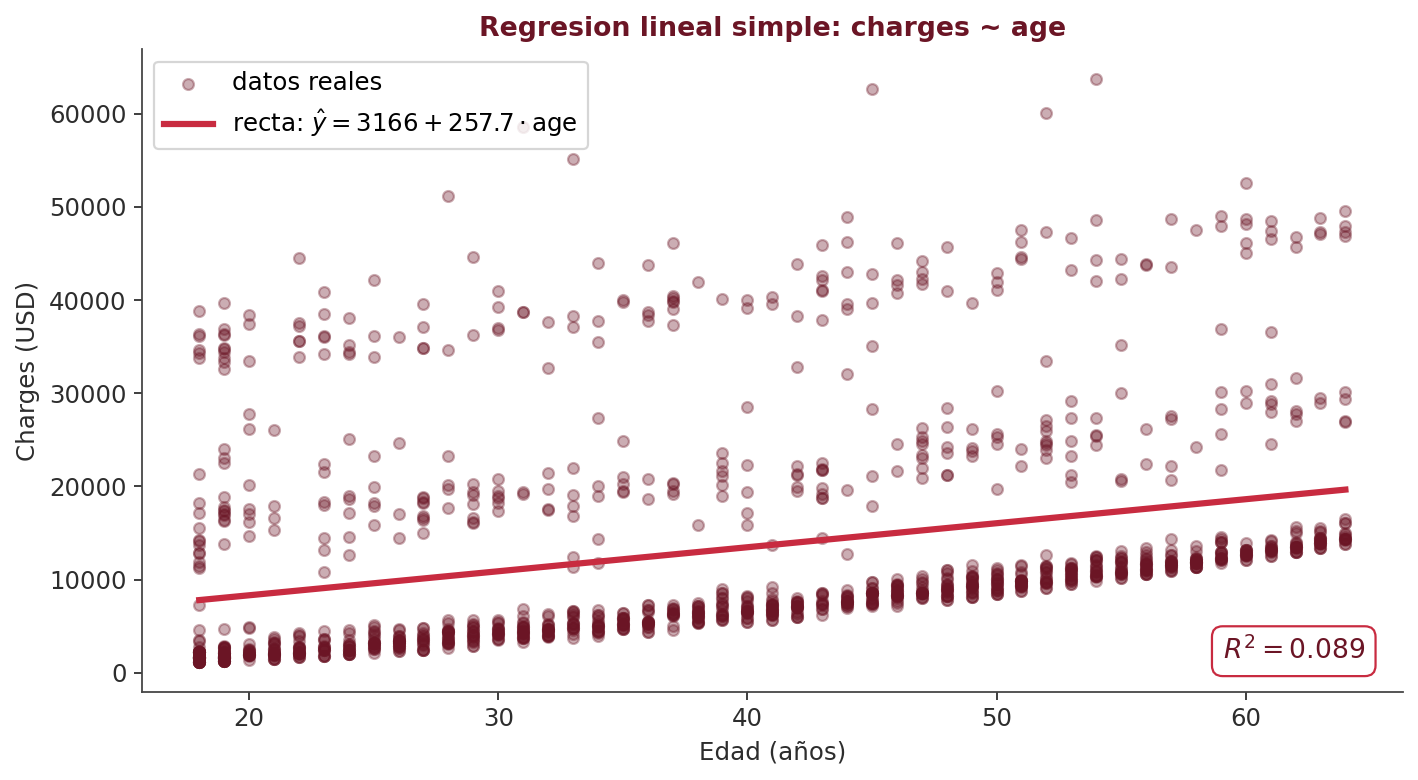
\includegraphics[width=0.78\textwidth]{img_regresion_simple.png}
  \end{center}

  \vspace{2pt}
  {\scriptsize\color{textMuted}
  \begin{itemize}\setlength{\itemsep}{2pt}
    \item[{\color{arcaRed}\scriptsize\faArrowRight}]
      La tendencia es clara: a más edad, más costo. Pero la recta deja
      \textbf{muchísimo error} sin explicar.
    \item[{\color{arcaRed}\scriptsize\faArrowRight}]
      ¿Las tres ``bandas'' que se ven? Son fumadores vs no fumadores
      --- el modelo no lo sabe todavía.
  \end{itemize}
  }
\end{frame}

\begin{frame}{¿Cómo Medimos Qué Tan Bueno Es?}
  \vspace{-4pt}
  {\footnotesize\color{arcaDark}\bfseries
    Tenemos una recta. Tenemos predicciones. Pero ¿cómo \textbf{ponemos un
    número} a qué tan equivocado está el modelo?}

  \vspace{6pt}
  \begin{center}
    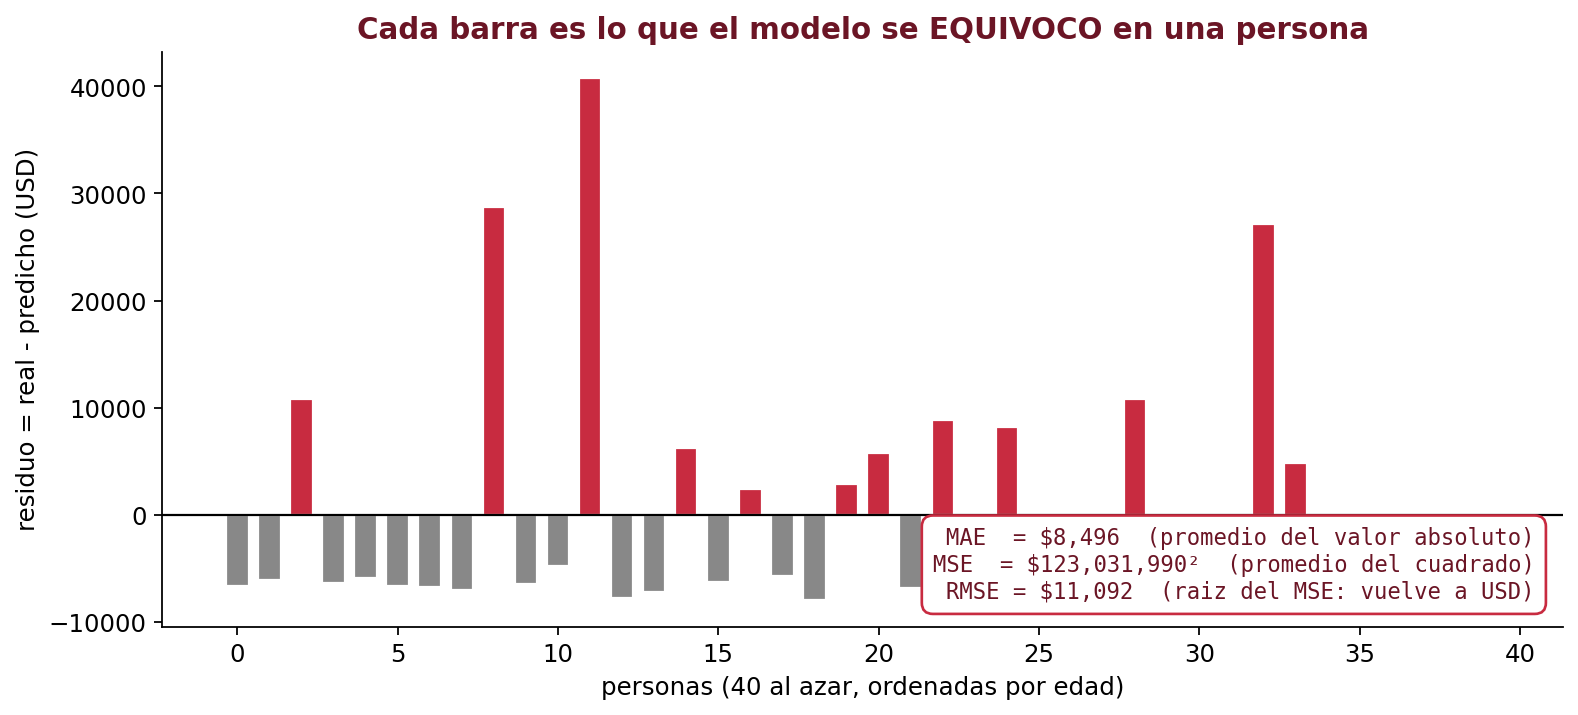
\includegraphics[width=0.78\textwidth]{img_residuos_barras.png}
  \end{center}

  \vspace{-2pt}
  {\scriptsize\color{textMuted}
  \begin{itemize}\setlength{\itemsep}{2pt}
    \item[{\color{arcaRed}\scriptsize\faArrowRight}]
      Cada barra es un \textbf{residuo}: la diferencia entre el valor
      real y el predicho.
    \item[{\color{arcaRed}\scriptsize\faArrowRight}]
      Hay barras positivas y negativas. Si las sumamos sin más,
      \textbf{se cancelan} y nos da casi 0 (lo cual no significa que
      el modelo sea perfecto).
    \item[{\color{arcaRed}\scriptsize\faArrowRight}]
      Necesitamos resumir esos residuos en \textbf{un solo número}.
      Hay tres formas estándar.
  \end{itemize}
  }
\end{frame}

\begin{frame}[shrink=5]{MSE --- Error Cuadrático Medio}
  \vspace{-4pt}
  {\footnotesize\color{arcaDark}\bfseries
    El más matemático de los tres. Y el que el modelo \textit{ya está}
    minimizando bajo el capó.}

  \vspace{6pt}
  \begin{center}
    \begin{tcolorbox}[colback=arcaGray, colframe=arcaRed, boxrule=1pt,
                      arc=4pt, width=0.62\textwidth]
    \centering
    \large
    $\text{MSE} = \dfrac{1}{n}\sum_{i=1}^{n}(y_i - \hat{y}_i)^2$
    \end{tcolorbox}
  \end{center}

  \vspace{6pt}
  {\scriptsize
  \begin{itemize}\setlength{\itemsep}{5pt}
    \item[{\color{arcaRed}\faArrowRight}]
      Promedio del \textbf{cuadrado} de los residuos.
    \item[{\color{arcaRed}\faArrowRight}]
      \textbf{¿Por qué al cuadrado?} Dos razones:
      \begin{itemize}
        \item Para que residuos positivos y negativos \textbf{no se cancelen}.
        \item Para \textbf{castigar más} los errores grandes (un error de
          \$1000 cuenta 100 veces más que uno de \$100).
      \end{itemize}
    \item[{\color{codeOrange}\faExclamationTriangle}]
      \textbf{Recuerdan los mínimos cuadrados?} El modelo OLS \textit{ya
      está} ajustando la recta para minimizar exactamente esto. MSE no
      es una métrica nueva: es \textbf{la cosa misma que el modelo está
      optimizando}.
  \end{itemize}
  }
\end{frame}

\begin{frame}[shrink=5]{RMSE y MAE --- Las Versiones Legibles}
  \vspace{-4pt}
  {\footnotesize\color{arcaDark}\bfseries
    MSE tiene un problema: está en \textbf{dólares al cuadrado}. Nadie
    sabe leer eso. Lo arreglamos de dos formas.}

  \vspace{6pt}
  \begin{columns}[T]
    \begin{column}{0.48\textwidth}
      \begin{center}
        \begin{tcolorbox}[colback=arcaGray, colframe=arcaRed, boxrule=0.8pt,
                          arc=3pt, width=\textwidth]
        \centering
        \footnotesize
        $\text{RMSE} = \sqrt{\text{MSE}} = \sqrt{\dfrac{1}{n}\sum(y_i - \hat{y}_i)^2}$
        \end{tcolorbox}
      \end{center}
      \vspace{4pt}
      {\scriptsize
      \begin{itemize}\setlength{\itemsep}{4pt}
        \item Tomamos la \textbf{raíz cuadrada} del MSE.
        \item \textbf{Vuelve a estar en dólares} (\$).
        \item Sigue castigando más los errores grandes.
        \item ``El modelo se equivoca en $\approx$ \$5\,800 por persona.''
      \end{itemize}
      }
    \end{column}

    \begin{column}{0.48\textwidth}
      \begin{center}
        \begin{tcolorbox}[colback=arcaGray, colframe=arcaRed, boxrule=0.8pt,
                          arc=3pt, width=\textwidth]
        \centering
        \footnotesize
        $\text{MAE} = \dfrac{1}{n}\sum |y_i - \hat{y}_i|$
        \end{tcolorbox}
      \end{center}
      \vspace{4pt}
      {\scriptsize
      \begin{itemize}\setlength{\itemsep}{4pt}
        \item Promedio del \textbf{valor absoluto}.
        \item También en dólares (\$).
        \item Trata todos los errores por igual.
        \item ``El modelo se equivoca en $\approx$ \$4\,200 por persona.''
      \end{itemize}
      }
    \end{column}
  \end{columns}

  \vspace{6pt}
  {\footnotesize\color{arcaDark}
    \faLightbulb\hspace{4pt}
    \textbf{En la práctica}: reporta \textbf{MAE} a no técnicos (más
    fácil de explicar) y \textbf{RMSE} cuando los errores grandes te
    importan más.}
\end{frame}

\begin{frame}{Pero Esperen: ¿\$5\,800 Es Mucho o Poco?}
  \vspace{-4pt}
  {\footnotesize\color{arcaDark}\bfseries
    RMSE = \$5\,800 suena alto. ¿Pero comparado con qué?}

  \vspace{8pt}
  {\footnotesize
  \begin{itemize}\setlength{\itemsep}{6pt}
    \item[{\color{arcaRed}\faArrowRight}]
      Necesitamos un \textbf{punto de comparación}. El más tonto posible:
      \textbf{predecir siempre la media} de \texttt{charges}.
    \item[{\color{arcaRed}\faArrowRight}]
      Ese es el \textbf{peor modelo razonable}: ignora todas las features
      y siempre dice ``\$13\,270''.
    \item[{\color{arcaRed}\faArrowRight}]
      Si nuestro modelo es \textbf{tan malo} como ese, no sirve para nada.
    \item[{\color{arcaRed}\faArrowRight}]
      Si nuestro modelo es \textbf{mucho mejor} que ese, vale la pena.
    \item[{\color{arcaRed}\faArrowRight}]
      Esa \textbf{comparación} es exactamente lo que mide R\textsuperscript{2}.
  \end{itemize}
  }
\end{frame}

\begin{frame}{R\textsuperscript{2}: La Comparación con el Modelo Tonto}
  \vspace{-4pt}
  {\footnotesize\color{arcaDark}\bfseries
    Comparemos visualmente: el modelo tonto (izquierda) vs nuestra
    regresión (derecha). Las líneas son los residuos.}

  \vspace{4pt}
  \begin{center}
    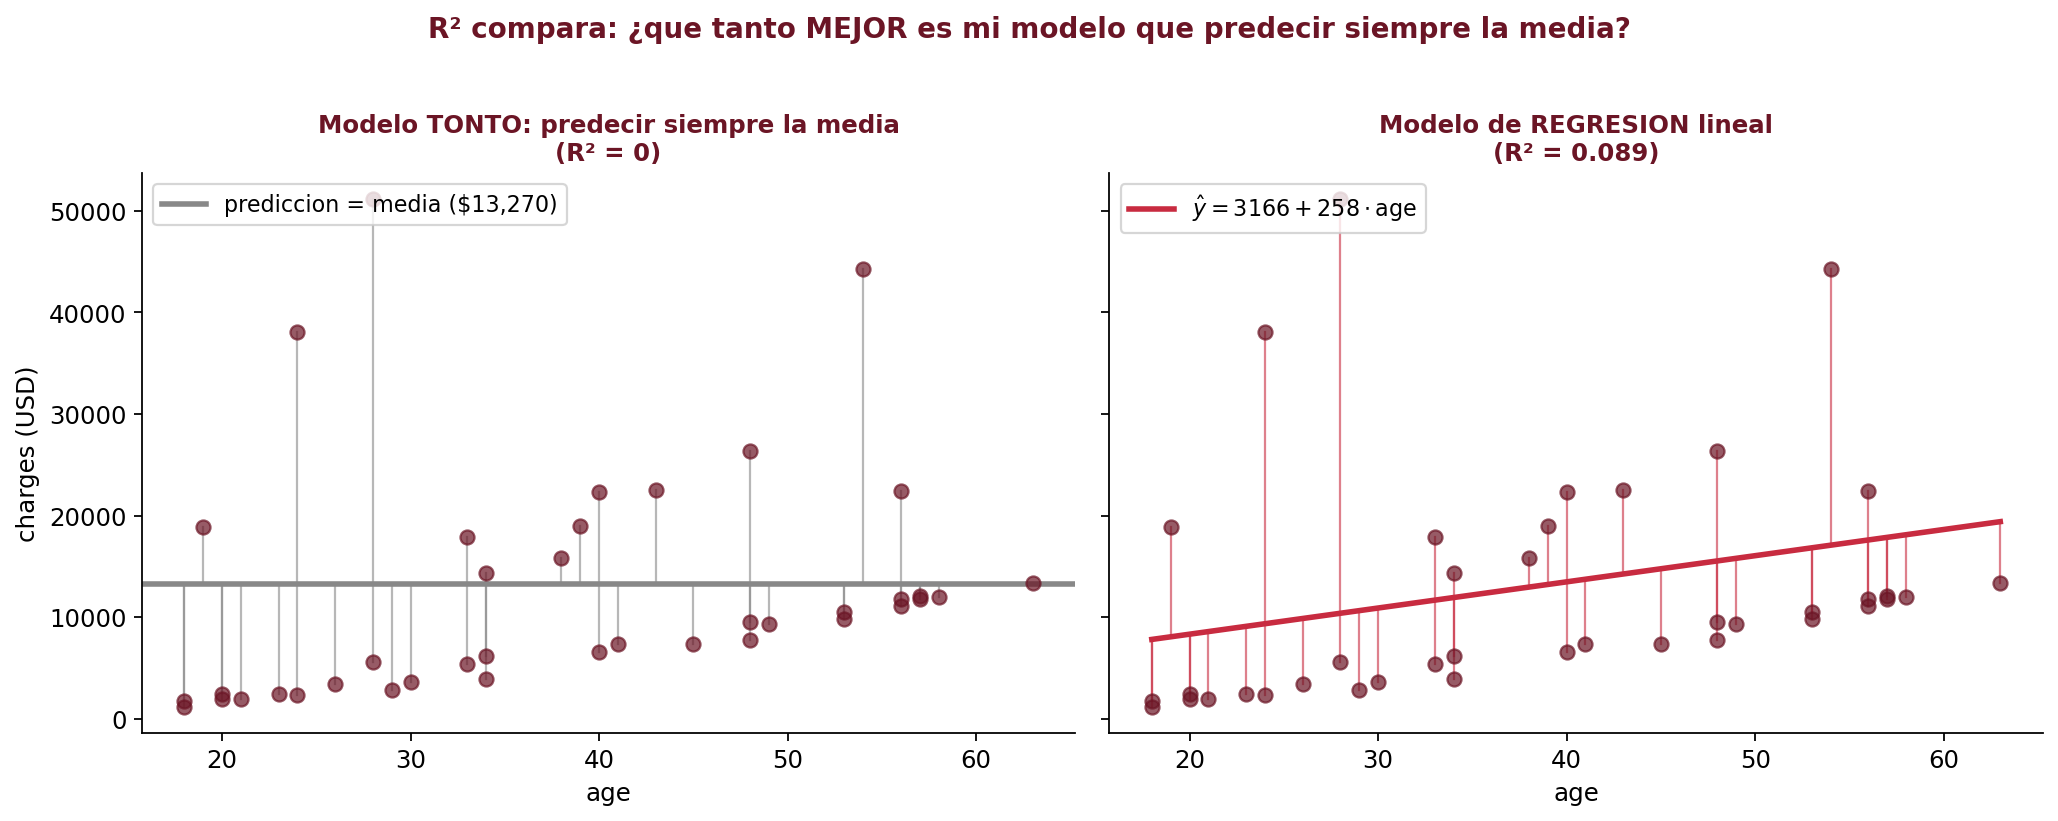
\includegraphics[width=0.95\textwidth]{img_r2_baseline.png}
  \end{center}

  \vspace{2pt}
  {\scriptsize\color{textMuted}
  \begin{itemize}\setlength{\itemsep}{2pt}
    \item[{\color{arcaRed}\scriptsize\faArrowRight}]
      Visualmente: los residuos del panel derecho (rojos) son
      \textbf{ligeramente más cortos} que los del izquierdo (grises).
    \item[{\color{arcaRed}\scriptsize\faArrowRight}]
      Esa pequeña mejora es lo que R\textsuperscript{2} mide.
  \end{itemize}
  }
\end{frame}

\begin{frame}{R\textsuperscript{2}: La Fórmula y Su Interpretación}
  \vspace{-4pt}
  {\footnotesize\color{arcaDark}\bfseries
    R\textsuperscript{2} es exactamente esa comparación, expresada como una fracción.}

  \vspace{10pt}
  \begin{center}
    \begin{tcolorbox}[colback=arcaGray, colframe=arcaRed, boxrule=1pt,
                      arc=4pt, width=0.7\textwidth]
    \centering
    \large
    $R^2 = 1 - \dfrac{\text{MSE del modelo}}{\text{MSE del modelo tonto}}$
    \end{tcolorbox}
  \end{center}

  \vspace{12pt}
  {\footnotesize
  \begin{itemize}\setlength{\itemsep}{8pt}
    \item[{\color{arcaRed}\faArrowRight}]
      \textbf{R\textsuperscript{2} = 0}: el modelo es \textbf{igual de malo}
      que predecir siempre la media. \textit{No aporta nada.}
    \item[{\color{arcaRed}\faArrowRight}]
      \textbf{R\textsuperscript{2} = 1}: el modelo es \textbf{perfecto}
      (MSE = 0, todos los residuos son cero).
    \item[{\color{arcaRed}\faArrowRight}]
      \textbf{R\textsuperscript{2} = 0.7}: el modelo \textbf{eliminó el 70\,\%}
      del error que tendría el modelo tonto.
  \end{itemize}
  }

  \vspace{8pt}
  {\footnotesize\color{arcaDark}
    \faLightbulb\hspace{4pt}
    Ahora R\textsuperscript{2} ya no es abstracto: es literalmente
    ``\textit{qué tanto mejor soy que la opción más tonta}''.}
\end{frame}

\begin{frame}[fragile,shrink=46]{Las 4 Métricas en Código}
  \vspace{-6pt}
  {\footnotesize\color{arcaDark}\bfseries
    Las cuatro juntas, para nuestro modelo simple (\texttt{charges} en función de \texttt{age}).}

  \vspace{4pt}
  \begin{pyblock}
from sklearn.metrics import (
    mean_squared_error, mean_absolute_error, r2_score
)

y_pred = modelo.predict(X_simple)

mse  = mean_squared_error(y, y_pred)
rmse = np.sqrt(mse)
mae  = mean_absolute_error(y, y_pred)
r2   = r2_score(y, y_pred)

print(f"MSE  = {mse:15,.0f}   (USD al cuadrado)")
print(f"RMSE = {rmse:15,.0f}   (USD)")
print(f"MAE  = {mae:15,.0f}   (USD)")
print(f"R2   = {r2:15.4f}")
  \end{pyblock}

  \vspace{4pt}
  \begin{outputblock}
MSE  =     132,481,544   (USD al cuadrado)
RMSE =          11,510   (USD)
MAE  =           9,090   (USD)
R2   =          0.0894
  \end{outputblock}
\end{frame}

\begin{frame}[shrink=5]{Lectura de Nuestro Modelo Simple}
  \vspace{-4pt}
  {\footnotesize\color{arcaDark}\bfseries
    Tradujamos los 4 números a frases de negocio.}

  \vspace{8pt}
  {\scriptsize
  \begin{itemize}\setlength{\itemsep}{6pt}
    \item[{\color{arcaRed}\faArrowRight}]
      \textbf{MAE = \$9\,090}: ``en promedio, el modelo se equivoca en \$9\,090
      al predecir el seguro de una persona''. \textbf{Mucho.}
    \item[{\color{arcaRed}\faArrowRight}]
      \textbf{RMSE = \$11\,510}: ``cuando se equivoca \textit{feo}, se
      equivoca por más de \$11\,000''. Aún peor.
    \item[{\color{arcaRed}\faArrowRight}]
      \textbf{R\textsuperscript{2} = 0.089}: ``mi modelo solo eliminó el
      \textbf{8.9\,\%} del error que tendría predecir siempre la media''. Casi nada.
  \end{itemize}
  }

  \vspace{6pt}
  {\footnotesize\color{arcaDark}
    \faLightbulb\hspace{4pt}
    Las 4 métricas dicen lo mismo con palabras distintas: \textbf{el modelo
    simple no sirve}. La edad sola no alcanza para predecir el seguro.\\
    \textbf{Solución}: agregar más variables. \textbf{Regresión múltiple.}}
\end{frame}

\begin{frame}[shrink=8]{Resumen: Cómo Leer Cada Métrica}
  \vspace{-4pt}
  {\footnotesize\color{arcaDark}\bfseries
    Tabla de referencia para cuando estén modelando solos.}

  \vspace{6pt}
  {\scriptsize
  \begin{tabular}{@{}lllp{6.4cm}@{}}
    \toprule
    \textbf{Métrica} & \textbf{Unidad} & \textbf{Rango} & \textbf{Cómo se lee} \\
    \midrule
    \textbf{MSE} & USD$^2$ & $[0, \infty)$ &
      ``Error cuadrático promedio''. Difícil de leer en negocio.
      Es la cantidad que el modelo \textbf{minimiza}. \\[3pt]
    \textbf{RMSE} & USD & $[0, \infty)$ &
      ``Cuando el modelo se equivoca \textit{feo}, falla por
      $\approx$ \$X''. Castiga más los errores grandes. \\[3pt]
    \textbf{MAE} & USD & $[0, \infty)$ &
      ``En promedio, el modelo se equivoca en \$X''. Trata todos
      los errores por igual. La más fácil de explicar. \\[3pt]
    \textbf{R\textsuperscript{2}} & sin unidad & $(-\infty, 1]$ &
      ``El modelo eliminó el X\,\% del error que tendría predecir
      siempre la media''. Score relativo, sin unidades. \\
    \bottomrule
  \end{tabular}
  }

  \vspace{8pt}
  {\footnotesize\color{arcaDark}
    \faLightbulb\hspace{4pt}
    \textbf{Comparación útil}: si \textbf{RMSE $\gg$ MAE}, hay errores grandes
    aislados (outliers en los residuos). Si \textbf{RMSE $\approx$ MAE}, los
    errores son uniformes.}
\end{frame}

\begin{frame}[shrink=10]{¿Cuándo Usar Cada Una?}
  \vspace{-4pt}
  {\footnotesize\color{arcaDark}\bfseries
    No hay una métrica ``correcta''. Depende del contexto y del público.}

  \vspace{6pt}
  {\scriptsize
  \begin{tabular}{@{}lp{5.5cm}p{5cm}@{}}
    \toprule
    \textbf{Métrica} & \textbf{Cuándo SÍ usarla} & \textbf{Cuándo NO} \\
    \midrule
    \textbf{MAE} &
      Reportes a no técnicos. Cuando todos los errores deben pesar igual.
      Cuando hay outliers que no quieres que dominen la métrica. &
      Cuando errores grandes son \textit{mucho} más caros que los
      pequeños. \\[3pt]
    \textbf{RMSE} &
      Cuando errores grandes son críticos (medicina, finanzas, predicción
      de demanda). Para presentar resultados técnicos. &
      Cuando hay outliers extremos que distorsionan: lo van a inflar. \\[3pt]
    \textbf{MSE} &
      Como \textit{loss function} interna. En papers académicos.
      Para optimizar el modelo (es lo que OLS minimiza). &
      Para reportar a humanos: las unidades al cuadrado son ilegibles. \\[3pt]
    \textbf{R\textsuperscript{2}} &
      Para \textbf{comparar modelos} sobre el mismo dataset.
      Para resúmenes ejecutivos (``el modelo explica el 78\,\%''). &
      Para comparar modelos en \textbf{datasets distintos}: un
      R\textsuperscript{2} de 0.4 puede ser excelente en un dominio
      y malísimo en otro. \\
    \bottomrule
  \end{tabular}
  }

  \vspace{8pt}
  {\footnotesize\color{arcaDark}
    \faLightbulb\hspace{4pt}
    \textbf{Combo recomendado para reportar}: \textbf{MAE} (en USD, fácil
    de explicar) \textbf{+ R\textsuperscript{2}} (score sin unidades para
    comparar modelos). Con esos dos cubres ejecutivos y científicos.}
\end{frame}

% =============================================================================
%  SECCIÓN 3: REGRESIÓN MÚLTIPLE
% =============================================================================
\sectionframe{De Una a Muchas Variables}{Regresión múltiple}

\begin{frame}[shrink=5]{Una Variable Nunca Explica Todo}
  \vspace{-4pt}
  {\footnotesize\color{arcaDark}\bfseries
    El costo del seguro no depende solo de la edad. Depende de
    \textbf{varias cosas a la vez}.}

  \vspace{8pt}
  \begin{center}
    \begin{tcolorbox}[colback=arcaGray, colframe=arcaRed, boxrule=1pt,
                      arc=4pt, width=0.85\textwidth]
    \centering
    \large
    $\hat{y} = \beta_0 + \beta_1 x_1 + \beta_2 x_2 + \ldots + \beta_n x_n$
    \end{tcolorbox}
  \end{center}

  \vspace{6pt}
  {\footnotesize
  \begin{itemize}\setlength{\itemsep}{5pt}
    \item[{\color{arcaRed}\faArrowRight}]
      Cada variable $x_i$ tiene su propio coeficiente $\beta_i$.
    \item[{\color{arcaRed}\faArrowRight}]
      El intercepto $\beta_0$ sigue siendo el ``valor base''.
    \item[{\color{arcaRed}\faArrowRight}]
      La matemática es la misma: minimizar la suma de residuos al cuadrado.
    \item[{\color{arcaRed}\faArrowRight}]
      \texttt{sklearn} \textbf{ni siquiera distingue} entre simple y múltiple:
      le pasas más columnas en \texttt{X} y ya.
  \end{itemize}
  }
\end{frame}

\begin{frame}[shrink=8]{``Manteniendo lo Demás Constante''}
  \vspace{-4pt}
  {\footnotesize\color{arcaDark}\bfseries
    El concepto más malentendido de toda la regresión múltiple.
    Vale la pena pelearlo.}

  \vspace{6pt}
  {\footnotesize
  Cuando decimos ``\textit{el coeficiente de} \texttt{age} \textit{es} 257'',
  significa:}

  \vspace{4pt}
  \begin{center}
    \begin{tcolorbox}[colback=arcaGray, colframe=arcaRed, boxrule=0.8pt,
                      arc=3pt, width=0.85\textwidth]
    \centering
    \footnotesize
    \textit{``Por cada año adicional de edad, el costo sube \$257,
    \textbf{manteniendo bmi, sex, smoker y region constantes}.''}
    \end{tcolorbox}
  \end{center}

  \vspace{6pt}
  {\scriptsize
  \begin{itemize}\setlength{\itemsep}{5pt}
    \item[{\color{arcaRed}\faArrowRight}]
      Es como comparar dos personas \textbf{idénticas en todo}
      excepto en la edad.
    \item[{\color{arcaRed}\faArrowRight}]
      Por eso los coeficientes \textbf{cambian} cuando agregas o
      quitas variables: el ``contexto'' cambia.
    \item[{\color{arcaRed}\faArrowRight}]
      En inglés: ``\textit{ceteris paribus}'' o
      ``\textit{controlling for the other variables}''.
  \end{itemize}
  }
\end{frame}

\begin{frame}[fragile,shrink=33]{Categóricas en Regresión: Encoding}
  \vspace{-6pt}
  {\footnotesize\color{arcaDark}\bfseries
    \textit{sklearn} no entiende texto. Recordamos clase 12: One-Hot Encoding.}

  \vspace{4pt}
  \begin{pyblock}
# Convertir las 3 categóricas a numéricas
df_enc = pd.get_dummies(
    df,
    columns=["sex", "smoker", "region"],
    drop_first=True,   # evita redundancia
    dtype=int
)
print(df_enc.columns.tolist())
  \end{pyblock}

  \vspace{4pt}
  \begin{outputblock}
Columnas resultantes (9):
  age, bmi, children, charges,
  sex_male, smoker_yes,
  region_northwest, region_southeast, region_southwest
  \end{outputblock}

  \vspace{4pt}
  {\scriptsize\color{textMuted}
  \begin{itemize}\setlength{\itemsep}{3pt}
    \item[{\color{arcaRed}\scriptsize\faArrowRight}]
      \texttt{drop\_first=True}: 4 regiones $\to$ solo 3 columnas (la cuarta se deduce).
  \end{itemize}
  }
\end{frame}

\begin{frame}[fragile,shrink=28]{Modelo Múltiple: Todas las Variables}
  \vspace{-6pt}
  {\footnotesize\color{arcaDark}\bfseries
    Mismo \texttt{LinearRegression}, ahora con \textbf{8 features}.}

  \vspace{4pt}
  \begin{pyblock}
X = df_enc.drop(columns=["charges"])
y = df_enc["charges"]

modelo_m = LinearRegression()
modelo_m.fit(X, y)

print(f"R^2: {modelo_m.score(X, y):.4f}")
print()
for nombre, coef in zip(X.columns, modelo_m.coef_):
    print(f"  {nombre:20s} {coef:12.2f}")
print(f"  {'intercepto':20s} {modelo_m.intercept_:12.2f}")
  \end{pyblock}
\end{frame}

\begin{frame}[fragile,shrink=28]{Salida del Modelo Múltiple}
  \vspace{-6pt}
  \begin{outputblock}
R^2: 0.7509

  age                    256.86
  bmi                    339.19
  children               475.50
  sex_male              -131.31
  smoker_yes           23848.53
  region_northwest      -353.00
  region_southeast      -1035.02
  region_southwest      -960.05
  intercepto          -11938.54
  \end{outputblock}

  \vspace{4pt}
  {\scriptsize\color{textMuted}
  \begin{itemize}\setlength{\itemsep}{3pt}
    \item[{\color{codeGreen}\scriptsize\faCheckCircle}]
      \textbf{R\textsuperscript{2} pasó de 0.09 a 0.75}. Brutal mejora.
    \item[{\color{codeOrange}\scriptsize\faExclamationTriangle}]
      \texttt{smoker\_yes = 23\,848}: \textbf{fumar suma \$24\,000} al seguro.
    \item[{\color{arcaRed}\scriptsize\faArrowRight}]
      Es el coeficiente más grande del modelo --- y por mucho.
  \end{itemize}
  }
\end{frame}

\begin{frame}[shrink=5]{El Coeficiente de \texttt{smoker\_yes}}
  \vspace{-4pt}
  {\footnotesize\color{arcaDark}\bfseries
    Este número es la mejor lección de regresión múltiple de toda la clase.}

  \vspace{8pt}
  \begin{center}
    \begin{tcolorbox}[colback=arcaGray, colframe=arcaRed, boxrule=1pt,
                      arc=4pt, width=0.7\textwidth]
    \centering
    $\beta_{\text{smoker\_yes}} = +23\,848$
    \end{tcolorbox}
  \end{center}

  \vspace{6pt}
  {\footnotesize
  \begin{itemize}\setlength{\itemsep}{5pt}
    \item[{\color{arcaRed}\faArrowRight}]
      \textbf{Lectura literal:} ``ser fumador (\texttt{smoker\_yes}=1)
      en lugar de no fumador (\texttt{smoker\_yes}=0) suma
      \textbf{\$23\,848} al seguro \textit{ceteris paribus}.''
    \item[{\color{arcaRed}\faArrowRight}]
      \textbf{Lectura de negocio:} dos personas idénticas en edad,
      bmi, sexo, hijos y región --- pero una fuma --- pagarán
      \textbf{\$24\,000 de diferencia} al año.
    \item[{\color{arcaRed}\faArrowRight}]
      Esto es lo que significa el coeficiente de una \textbf{dummy}
      en una regresión: el ``salto'' que produce esa categoría
      respecto a la de referencia.
  \end{itemize}
  }
\end{frame}

\begin{frame}[shrink=5]{Pero Espera: ¿Cuál Variable Importa Más?}
  \vspace{-4pt}
  {\footnotesize\color{arcaDark}\bfseries
    Pregunta natural --- y trampa clásica. Veamos los coeficientes:}

  \vspace{6pt}
  {\scriptsize
  \begin{tabular}{@{}lrl@{}}
    \toprule
    \textbf{Variable} & \textbf{Coeficiente} & \textbf{Unidad} \\
    \midrule
    age & $+257$ & por año \\
    bmi & $+339$ & por unidad de BMI \\
    children & $+476$ & por hijo \\
    smoker\_yes & $+23\,848$ & 0/1 (fumar o no) \\
    \bottomrule
  \end{tabular}
  }

  \vspace{6pt}
  {\footnotesize\color{arcaRed}\bfseries
    \faTimesCircle\hspace{4pt}
    No puedes comparar 257 con 23\,848 directamente.}
  \vspace{4pt}

  {\scriptsize
  Las unidades son distintas: ``año'' no es lo mismo que ``unidad de BMI''
  ni que ``binario 0/1''. Necesitas ponerlas todas en la \textbf{misma escala}
  antes de compararlas.}

  \vspace{6pt}
  {\footnotesize\color{arcaDark}
    \faLightbulb\hspace{4pt}
    \textbf{La solución}: \textit{estandarización}. Y la fórmula que vamos
    a usar... ya la conocen.}
\end{frame}

% =============================================================================
%  SECCIÓN 4: ESTANDARIZACIÓN
% =============================================================================
\sectionframe{Estandarización}{El z-score reaparece, esta vez con otro propósito}

\begin{frame}{El Problema, Visualizado}
  \vspace{-4pt}
  {\footnotesize\color{arcaDark}\bfseries
    Pongamos las 4 variables numéricas en el \textbf{mismo gráfico}.
    A ver qué pasa.}

  \vspace{2pt}
  \begin{center}
    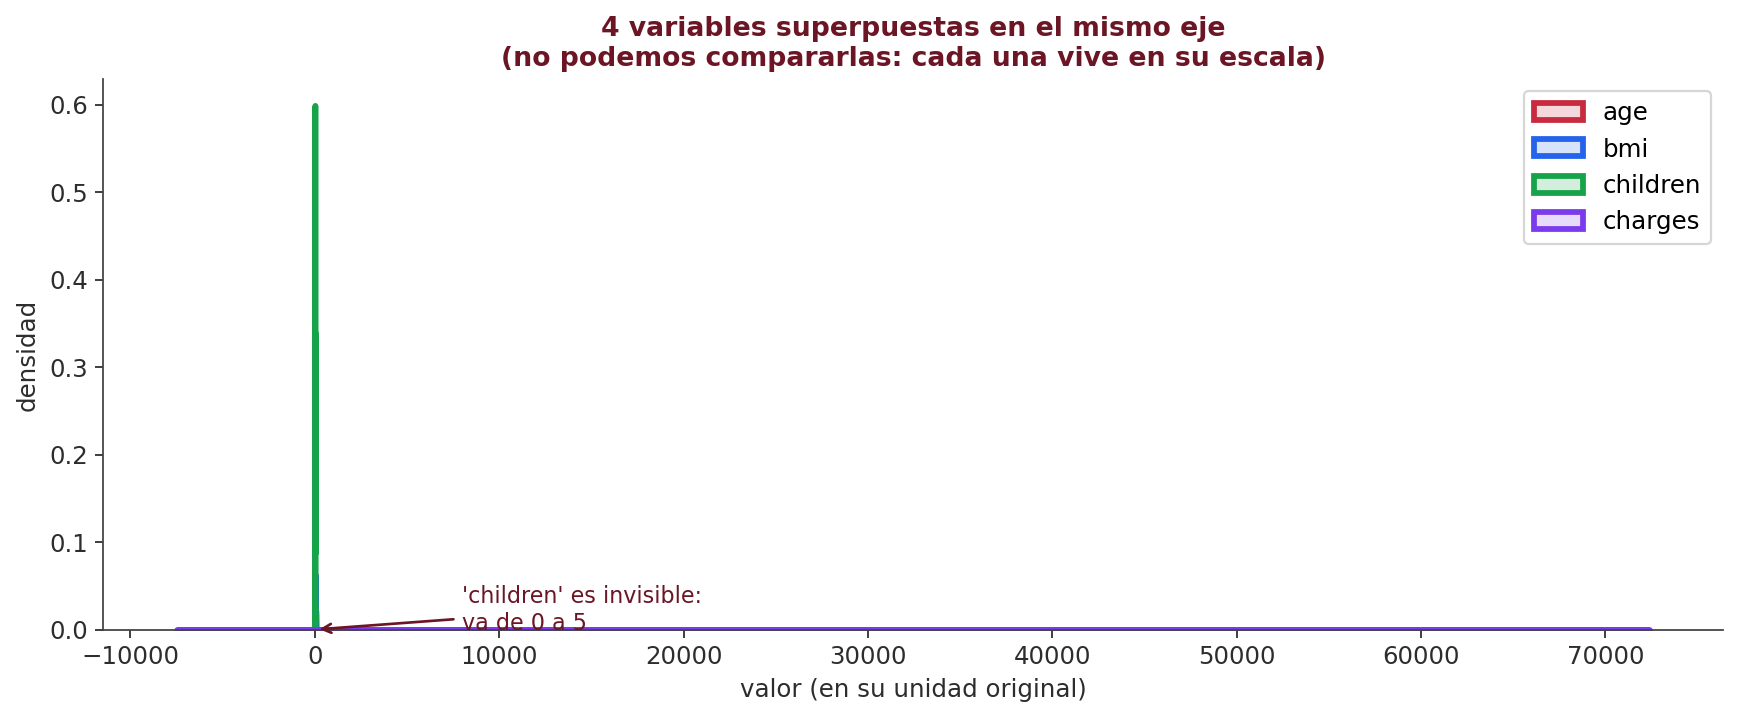
\includegraphics[width=0.78\textwidth]{img_dist_antes.png}
  \end{center}

  \vspace{-2pt}
  {\scriptsize\color{textMuted}
  \begin{itemize}\setlength{\itemsep}{2pt}
    \item[{\color{arcaRed}\scriptsize\faArrowRight}]
      \texttt{children} ni siquiera se ve --- su rango (0 a 5) es
      \textbf{microscópico} comparado con \texttt{charges} (0 a 64\,000).
    \item[{\color{arcaRed}\scriptsize\faArrowRight}]
      Es imposible compararlas. Cada una vive en su propio mundo.
  \end{itemize}
  }
\end{frame}

\begin{frame}{¿Por Qué Importa Esto?}
  \vspace{-4pt}
  {\footnotesize\color{arcaDark}\bfseries
    Cuando las features tienen escalas radicalmente distintas, dos cosas
    importantes se vuelven imposibles:}

  \vspace{8pt}
  \begin{columns}[T]
    \begin{column}{0.48\textwidth}
      {\footnotesize\bfseries\color{arcaRed}
        \faTimesCircle\hspace{4pt} Comparar la importancia
        de las variables}
      \vspace{4pt}

      {\scriptsize
      ¿Es ``+339 por unidad de BMI'' más o menos importante que
      ``+24\,000 por fumar''? Imposible saberlo: están en
      \textbf{unidades distintas}.}
    \end{column}

    \begin{column}{0.48\textwidth}
      {\footnotesize\bfseries\color{arcaRed}
        \faTimesCircle\hspace{4pt} Modelos sensibles a la escala}
      \vspace{4pt}

      {\scriptsize
      KNN, SVM, redes neuronales, k-means, regresión regularizada\dots
      todos miden \textbf{distancias}. Una variable de escala grande
      \textbf{domina} a las demás aunque no sea más importante.}
    \end{column}
  \end{columns}

  \vspace{8pt}
  {\footnotesize\color{arcaDark}
    \faLightbulb\hspace{4pt}
    \textbf{La solución}: poner todas las variables en la \textbf{misma
    escala}. Y la fórmula que usamos\dots\ ya la conocen desde clase 09.}
\end{frame}

\begin{frame}{El z-score: Misma Fórmula, Propósito Nuevo}
  \vspace{-4pt}
  {\footnotesize\color{arcaDark}\bfseries
    En clases 9 y 10 usaron esta fórmula para detectar outliers.
    Hoy la usan para preparar features. Veámosla aplicada a \texttt{age}.}

  \vspace{4pt}
  \begin{center}
    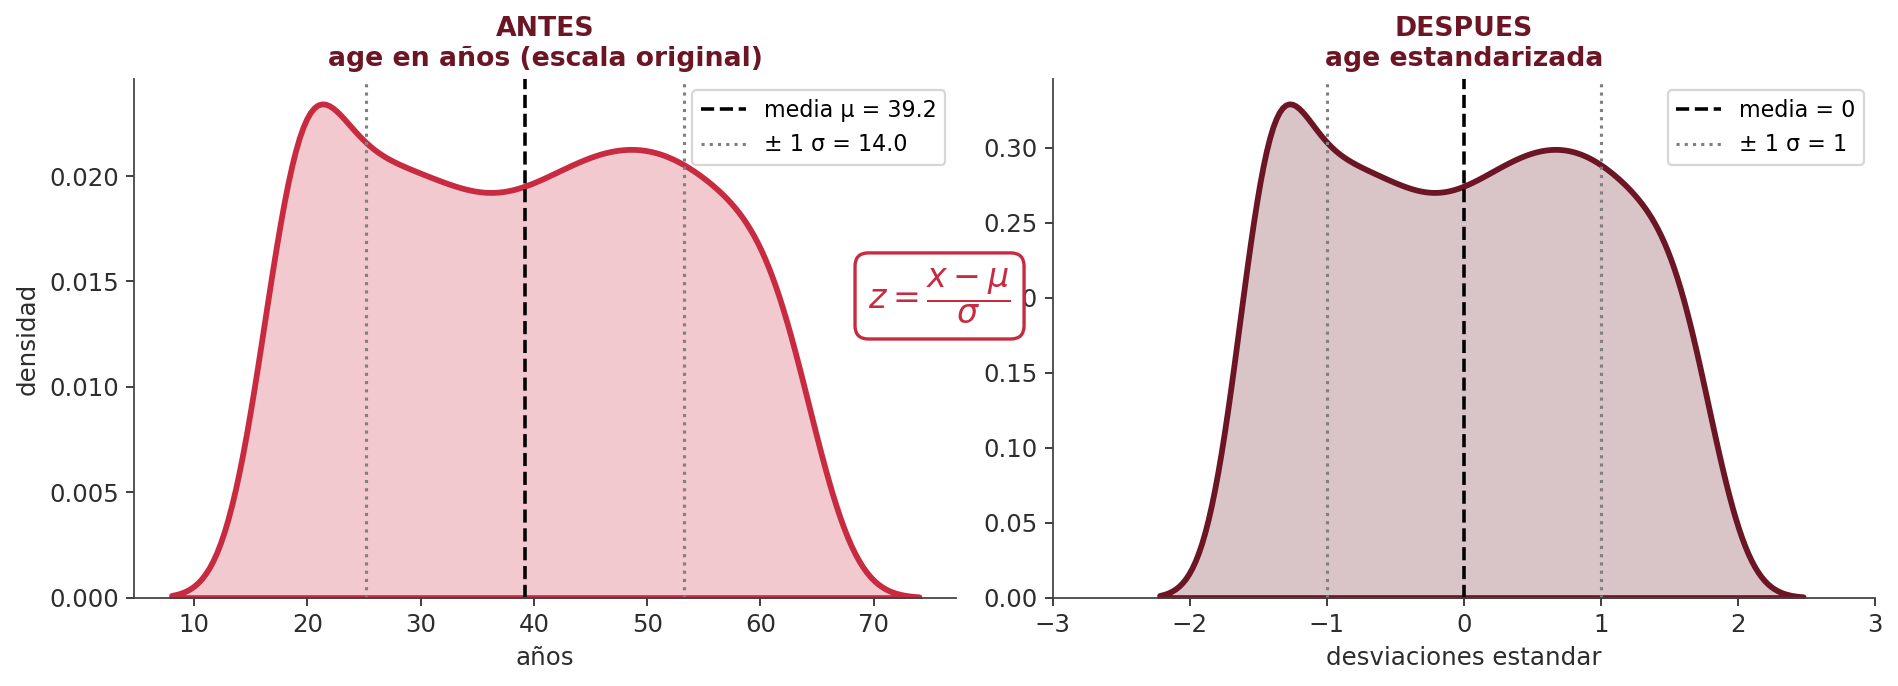
\includegraphics[width=0.90\textwidth]{img_zscore_pasos.png}
  \end{center}

  \vspace{-2pt}
  {\scriptsize\color{textMuted}
  \begin{itemize}\setlength{\itemsep}{2pt}
    \item[{\color{arcaRed}\scriptsize\faArrowRight}]
      \textbf{La forma de la distribución no cambia}. Solo cambia el eje.
    \item[{\color{arcaRed}\scriptsize\faArrowRight}]
      Después de la transformación, la media es 0 y \textbf{una unidad}
      en el eje significa \textbf{una desviación estándar}.
  \end{itemize}
  }
\end{frame}

\begin{frame}{Después de Estandarizar: Todas Visibles}
  \vspace{-4pt}
  {\footnotesize\color{arcaDark}\bfseries
    Aplicamos $z = (x - \mu) / \sigma$ a las 4 variables y volvemos a
    superponerlas en el mismo gráfico.}

  \vspace{2pt}
  \begin{center}
    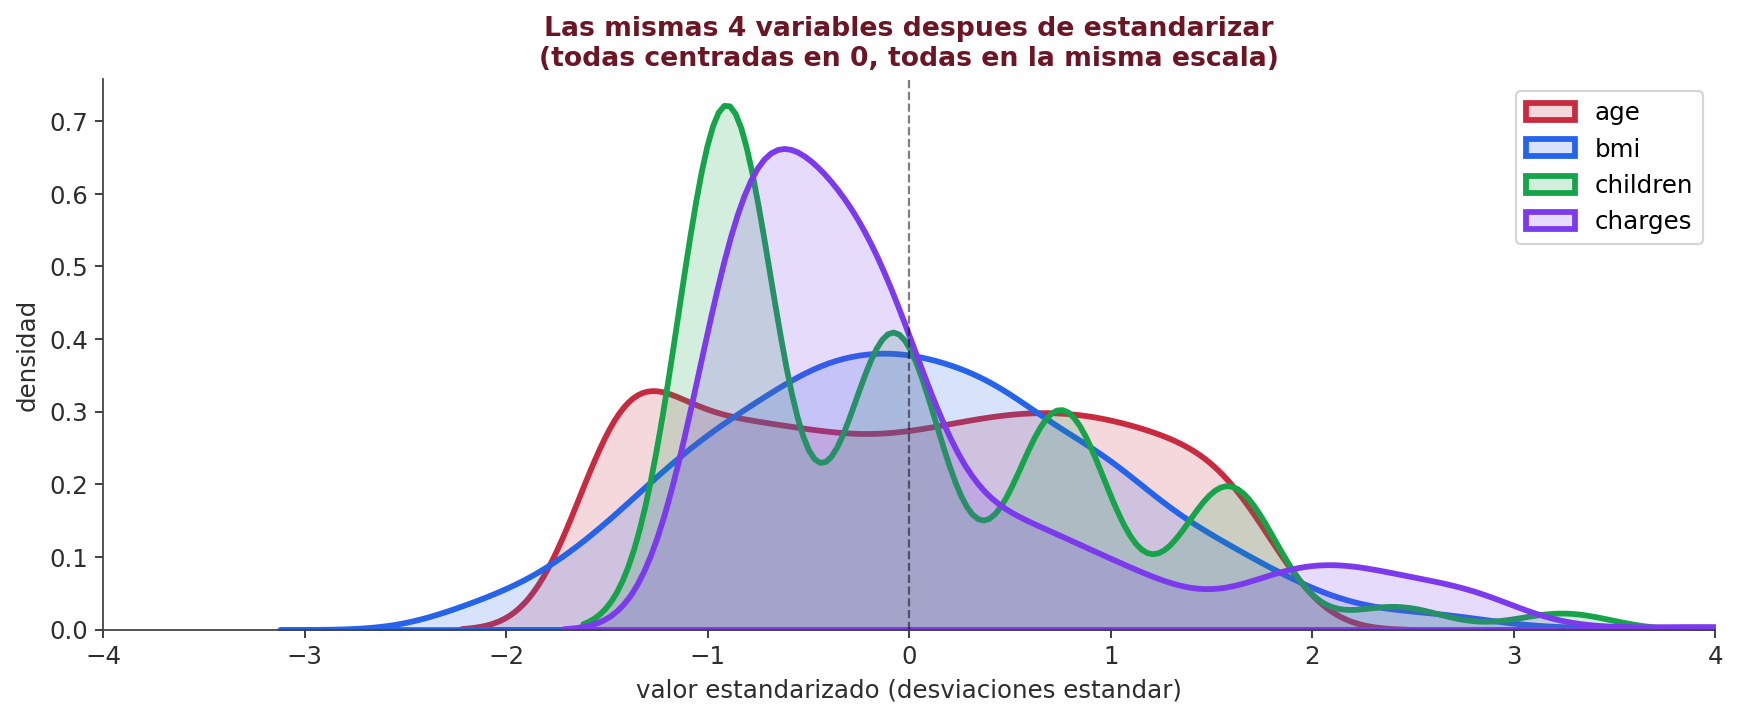
\includegraphics[width=0.78\textwidth]{img_dist_despues.png}
  \end{center}

  \vspace{-2pt}
  {\scriptsize\color{textMuted}
  \begin{itemize}\setlength{\itemsep}{2pt}
    \item[{\color{codeGreen}\scriptsize\faCheckCircle}]
      Ahora se ven \textbf{las cuatro}. Todas centradas en 0, todas
      en el mismo rango.
    \item[{\color{arcaRed}\scriptsize\faArrowRight}]
      ``1 unidad de age'' significa lo mismo que ``1 unidad de bmi'':
      \textbf{una desviación estándar}.
  \end{itemize}
  }
\end{frame}

\begin{frame}[fragile,shrink=28]{\texttt{StandardScaler} de sklearn}
  \vspace{-6pt}
  {\footnotesize\color{arcaDark}\bfseries
    sklearn implementa el z-score como transformador de features.}

  \vspace{4pt}
  \begin{pyblock}
from sklearn.preprocessing import StandardScaler

scaler = StandardScaler()
X_scaled = scaler.fit_transform(X)

# Comprobar: media ~0 y desviacion ~1 en cada columna
print(f"Medias:       {X_scaled.mean(axis=0).round(2)}")
print(f"Desviaciones: {X_scaled.std(axis=0).round(2)}")
  \end{pyblock}

  \vspace{4pt}
  \begin{outputblock}
Medias:       [-0.  0.  0. -0.  0.  0. -0.  0.]
Desviaciones: [1. 1. 1. 1. 1. 1. 1. 1.]
  \end{outputblock}
\end{frame}

\begin{frame}[fragile,shrink=28]{Modelo con Features Estandarizadas}
  \vspace{-6pt}
  {\footnotesize\color{arcaDark}\bfseries
    Mismo modelo, ahora con $X$ escalado. Los coeficientes serán comparables.}

  \vspace{4pt}
  \begin{pyblock}
modelo_std = LinearRegression().fit(X_scaled, y)

for nombre, coef in zip(X.columns, modelo_std.coef_):
    print(f"  {nombre:20s} {coef:10.2f}")
  \end{pyblock}

  \vspace{4pt}
  \begin{outputblock}
  age                    3608.06
  bmi                    2050.96
  children                572.69
  sex_male                -65.66
  smoker_yes             9617.35
  region_northwest        -75.36
  region_southeast        -222.07
  region_southwest        -206.63
  \end{outputblock}
\end{frame}

\begin{frame}{Ahora Sí: ¿Cuál Variable Importa Más?}
  \vspace{-4pt}
  {\footnotesize\color{arcaDark}\bfseries
    Con todas las features estandarizadas, los coeficientes ya son comparables.
    El ranking aparece solo.}

  \vspace{2pt}
  \begin{center}
    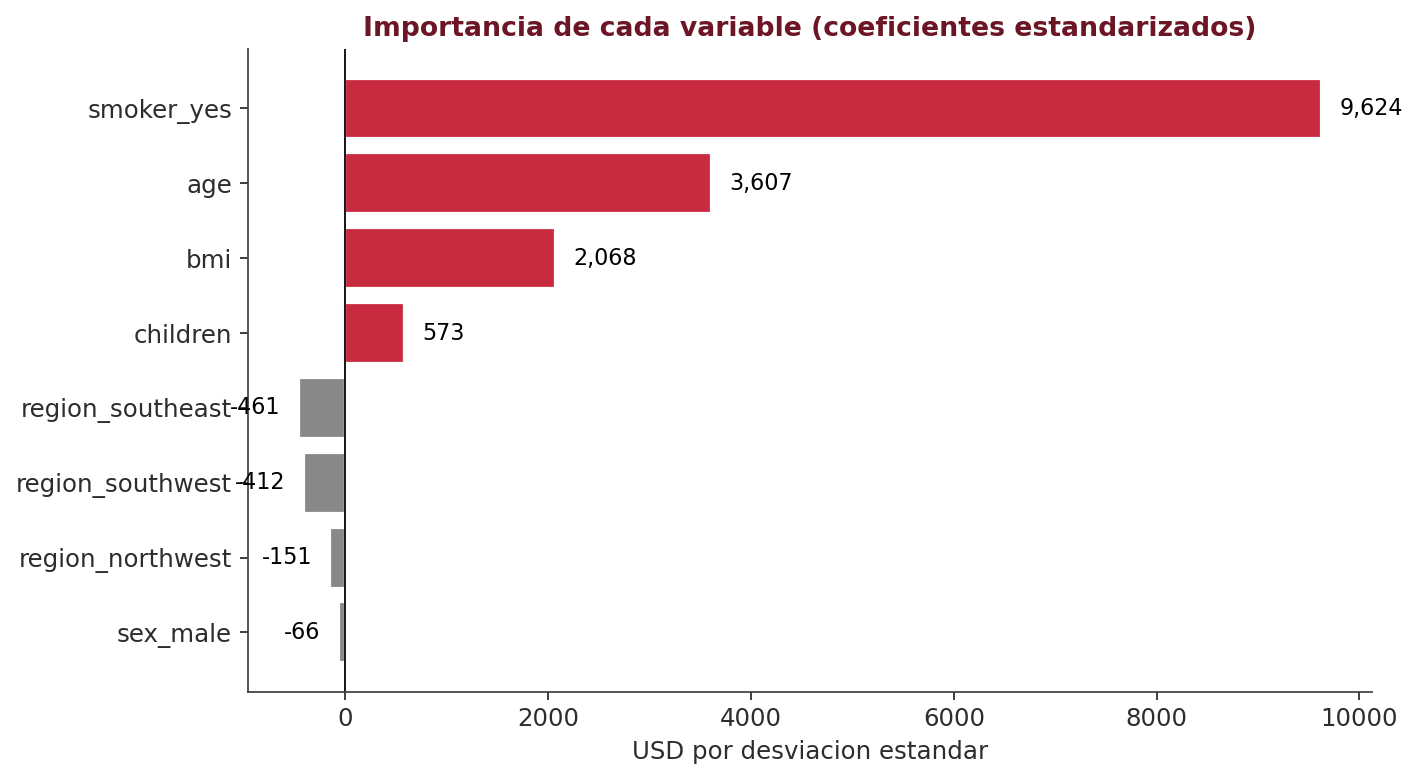
\includegraphics[width=0.78\textwidth]{img_coef_comparacion.png}
  \end{center}

  \vspace{-2pt}
  {\scriptsize\color{textMuted}
  \begin{itemize}\setlength{\itemsep}{2pt}
    \item[{\color{codeGreen}\scriptsize\faCheckCircle}]
      \textbf{Fumar} domina, seguido de \textbf{edad} y \textbf{BMI}. Sexo y
      región casi no importan.
    \item[{\color{codeOrange}\scriptsize\faExclamationTriangle}]
      Las predicciones del modelo \textbf{no cambian} al estandarizar. Solo
      cambia la \textbf{interpretación} de los coeficientes.
  \end{itemize}
  }
\end{frame}

\begin{frame}[shrink=8]{La Trampa: Data Leakage}
  \vspace{-4pt}
  {\footnotesize\color{arcaDark}\bfseries
    Cómo \textbf{NO} hacer estandarización. Error \#1 de principiantes.}

  \vspace{6pt}
  \begin{columns}[T]
    \begin{column}{0.48\textwidth}
      {\footnotesize\color{arcaRed}\bfseries\faTimesCircle\hspace{4pt}
        Mal:}
      \vspace{4pt}

      \begin{tcolorbox}[colback=arcaGray, colframe=arcaRed, boxrule=0.5pt,
                        arc=2pt, fontupper=\scriptsize\ttfamily]
scaler.fit(X\_completo)\\
X\_train\_s = scaler.transform(X\_train)\\
X\_test\_s  = scaler.transform(X\_test)
      \end{tcolorbox}

      \vspace{4pt}
      {\scriptsize\color{arcaRed}
      Calculas la media usando \textbf{también} los datos de test.
      Tu modelo ``conoce'' el futuro $\to$ evaluación inflada.}
    \end{column}

    \begin{column}{0.48\textwidth}
      {\footnotesize\color{codeGreen}\bfseries\faCheckCircle\hspace{4pt}
        Bien:}
      \vspace{4pt}

      \begin{tcolorbox}[colback=arcaGray, colframe=codeGreen, boxrule=0.5pt,
                        arc=2pt, fontupper=\scriptsize\ttfamily]
scaler.fit(X\_train)\\
X\_train\_s = scaler.transform(X\_train)\\
X\_test\_s  = scaler.transform(X\_test)
      \end{tcolorbox}

      \vspace{4pt}
      {\scriptsize\color{codeGreen}
      \texttt{fit} solo con train. \texttt{transform} en ambos
      con los parámetros aprendidos. El test queda intacto.}
    \end{column}
  \end{columns}

  \vspace{6pt}
  {\footnotesize\color{arcaDark}
    \faLightbulb\hspace{4pt}
    \textbf{Regla universal de ML}: cualquier transformación que
    aprenda parámetros (media, desviación, mínimos, máximos...) se
    \textbf{ajusta solo con los datos de entrenamiento}.}
\end{frame}

% =============================================================================
%  SECCIÓN 5: TRAIN / TEST SPLIT
% =============================================================================
\sectionframe{Train / Test Split}{¿Cómo sé si mi modelo es bueno?}

\begin{frame}[shrink=5]{Pregunta Provocadora}
  \vspace{-4pt}
  {\footnotesize\color{arcaDark}\bfseries
    Acabamos de obtener R\textsuperscript{2} = 0.75. \textbf{¿Cómo sabemos
    que el modelo es bueno?}}

  \vspace{8pt}
  \begin{columns}[T]
    \begin{column}{0.48\textwidth}
      {\footnotesize\color{arcaRed}\bfseries\faTimesCircle\hspace{4pt}
        Respuesta intuitiva (errónea):}
      \vspace{4pt}

      {\scriptsize\color{textDark}
      ``\textit{R\textsuperscript{2} alto en mis datos $=$ buen modelo}.''
      }

      \vspace{6pt}
      {\scriptsize
      \begin{itemize}\setlength{\itemsep}{4pt}
        \item Calculé R\textsuperscript{2} \textbf{con los mismos datos}
          que usé para entrenar.
        \item Es como aprenderme las respuestas de un examen y luego
          ``aprobarlo'' contestando las mismas preguntas.
        \item No mide la capacidad de \textbf{generalizar} a datos nuevos.
      \end{itemize}
      }
    \end{column}

    \begin{column}{0.48\textwidth}
      {\footnotesize\color{codeGreen}\bfseries\faCheckCircle\hspace{4pt}
        Respuesta correcta:}
      \vspace{4pt}

      {\scriptsize\color{textDark}
      ``\textit{Probemos el modelo con datos que \textbf{nunca vio}}.''
      }

      \vspace{6pt}
      {\scriptsize
      \begin{itemize}\setlength{\itemsep}{4pt}
        \item Separamos los datos \textbf{antes} de entrenar.
        \item Una parte para \textbf{enseñar} (train).
        \item Otra parte, escondida, para \textbf{examinar}
          (test).
        \item El test simula ``datos del futuro'' que aún no existen.
      \end{itemize}
      }
    \end{column}
  \end{columns}
\end{frame}

\begin{frame}[fragile,shrink=28]{\texttt{train\_test\_split}}
  \vspace{-6pt}
  {\footnotesize\color{arcaDark}\bfseries
    La función más usada de todo \texttt{sklearn}.}

  \vspace{4pt}
  \begin{pyblock}
from sklearn.model_selection import train_test_split

X_train, X_test, y_train, y_test = train_test_split(
    X, y,
    test_size=0.2,      # 20% para test, 80% para train
    random_state=42     # reproducibilidad
)

print(f"Train: {X_train.shape[0]} filas")
print(f"Test:  {X_test.shape[0]} filas")
  \end{pyblock}

  \vspace{4pt}
  \begin{outputblock}
Train: 1070 filas
Test:  268 filas
  \end{outputblock}
\end{frame}

\begin{frame}[fragile,shrink=32]{Entrenar y Evaluar Correctamente}
  \vspace{-6pt}
  {\footnotesize\color{arcaDark}\bfseries
    \texttt{fit} solo con train. Evaluar con test.}

  \vspace{4pt}
  \begin{pyblock}
from sklearn.metrics import (
    r2_score, mean_absolute_error, mean_squared_error
)

modelo = LinearRegression().fit(X_train, y_train)

y_pred_train = modelo.predict(X_train)
y_pred_test  = modelo.predict(X_test)

print(f"R^2 train: {r2_score(y_train, y_pred_train):.4f}")
print(f"R^2 test : {r2_score(y_test,  y_pred_test):.4f}")
  \end{pyblock}

  \vspace{4pt}
  \begin{outputblock}
R^2 train: 0.7417
R^2 test : 0.7836
  \end{outputblock}
\end{frame}

\begin{frame}[fragile,shrink=42]{Las 4 Métricas en el Test Set}
  \vspace{-6pt}
  {\footnotesize\color{arcaDark}\bfseries
    Aplicamos las mismas 4 métricas, ahora sobre el modelo \textbf{múltiple}
    en \textbf{test}.}

  \vspace{4pt}
  \begin{pyblock}
y_pred_test = modelo.predict(X_test)

mse  = mean_squared_error(y_test, y_pred_test)
rmse = np.sqrt(mse)
mae  = mean_absolute_error(y_test, y_pred_test)
r2   = r2_score(y_test, y_pred_test)

print(f"MAE  test: {mae:10,.0f}  USD")
print(f"RMSE test: {rmse:10,.0f}  USD")
print(f"R2   test: {r2:11.4f}")
  \end{pyblock}

  \vspace{4pt}
  \begin{outputblock}
MAE  test:      4,181  USD
RMSE test:      5,796  USD
R2   test:     0.7836
  \end{outputblock}

  \vspace{4pt}
  {\scriptsize\color{textMuted}
  \begin{itemize}\setlength{\itemsep}{3pt}
    \item[{\color{codeGreen}\scriptsize\faCheckCircle}]
      \textbf{MAE pasó de \$9\,090 a \$4\,181} (modelo simple $\to$ múltiple).
      Mejora de más del 50\,\%.
    \item[{\color{codeGreen}\scriptsize\faCheckCircle}]
      \textbf{R\textsuperscript{2} pasó de 0.089 a 0.78}: ahora el modelo
      elimina el 78\,\% del error del modelo tonto.
  \end{itemize}
  }
\end{frame}

\begin{frame}{Predicho vs Real (en el Test Set)}
  \vspace{-4pt}
  {\footnotesize\color{arcaDark}\bfseries
    Cada punto es una persona del test. Mientras más cerca de la diagonal,
    mejor predijo el modelo.}

  \vspace{2pt}
  \begin{center}
    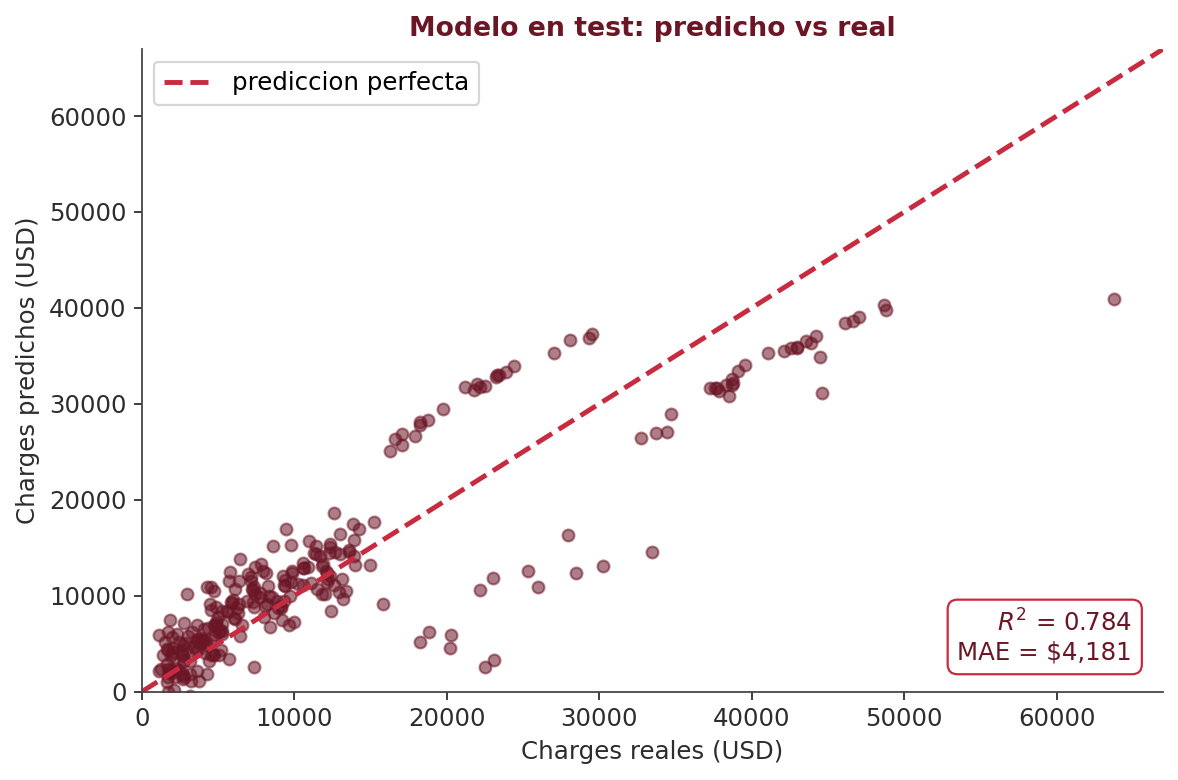
\includegraphics[width=0.62\textwidth]{img_predicho_vs_real.png}
  \end{center}

  \vspace{-2pt}
  {\scriptsize\color{textMuted}
  \begin{itemize}\setlength{\itemsep}{2pt}
    \item[{\color{codeGreen}\scriptsize\faCheckCircle}]
      La mayoría de puntos están \textbf{cerca de la diagonal} $\to$
      buenas predicciones.
    \item[{\color{codeOrange}\scriptsize\faExclamationTriangle}]
      Hay un grupo arriba a la izquierda donde el modelo \textbf{subestima}
      mucho: predijo \$10\,k pero la persona pagó \$40\,k+. Probablemente
      fumadores con condiciones adicionales que el modelo no captura.
  \end{itemize}
  }
\end{frame}

\begin{frame}[shrink=8]{Sobreajuste (\textit{Overfitting}): el Síntoma}
  \vspace{-4pt}
  {\footnotesize\color{arcaDark}\bfseries
    Compara siempre R\textsuperscript{2} en train vs test. Si difieren mucho,
    algo está mal.}

  \vspace{6pt}
  {\scriptsize
  \begin{tabular}{@{}lcl@{}}
    \toprule
    \textbf{Situación} & \textbf{Train vs Test} & \textbf{Diagnóstico} \\
    \midrule
    R\textsuperscript{2}\;train $\approx$ R\textsuperscript{2}\;test &
      0.74 vs 0.78 & \color{codeGreen}\bfseries Sano. Generaliza bien. \\
    R\textsuperscript{2}\;train $\gg$ R\textsuperscript{2}\;test &
      0.99 vs 0.40 & \color{arcaRed}\bfseries \textbf{Overfitting:} memorizó
        en lugar de aprender. \\
    R\textsuperscript{2}\;train $\approx$ R\textsuperscript{2}\;test (bajos) &
      0.20 vs 0.18 & \color{codeOrange}\bfseries \textbf{Underfitting:}
        modelo demasiado simple. \\
    \bottomrule
  \end{tabular}
  }

  \vspace{6pt}
  {\footnotesize
  \begin{itemize}\setlength{\itemsep}{4pt}
    \item[{\color{arcaRed}\faArrowRight}]
      Nuestro modelo: \textbf{0.74 train vs 0.78 test} $\to$ no hay overfitting.
    \item[{\color{arcaRed}\faArrowRight}]
      La regresión lineal es un modelo \textbf{poco propenso} a overfitting
      cuando hay pocas variables. Modelos más complejos
      (que veremos en Módulo 4) sí lo sufren mucho más.
  \end{itemize}
  }

  \vspace{4pt}
  {\footnotesize\color{arcaDark}
    \faLightbulb\hspace{4pt}
    \textbf{La palabra \textit{overfitting} la van a escuchar el resto del curso.}
    Memorícenla.}
\end{frame}

% =============================================================================
%  SECCIÓN 6: CIERRE
% =============================================================================
\sectionframe{Cierre}{Lo que acaban de hacer es Machine Learning}

\begin{frame}[shrink=5]{El Flujo que Aprendieron Hoy}
  \vspace{-4pt}
  {\footnotesize\color{arcaDark}\bfseries
    Este flujo --- exactamente este --- es el de \textbf{cualquier} modelo
    supervisado que verán en el resto del curso.}

  \vspace{8pt}
  \begin{center}
  \begin{tikzpicture}[
    node distance=0.4cm,
    box/.style={rectangle, rounded corners=4pt, draw=arcaRed, fill=arcaRed!8,
                minimum width=2.6cm, minimum height=0.9cm,
                font=\footnotesize\bfseries\color{arcaDark}, align=center},
    arr/.style={->, >=Stealth, thick, arcaRed},
  ]
    \node[box] (b1) {1. Split\\\scriptsize train/test};
    \node[box, right=of b1] (b2) {2. Encode\\\scriptsize categóricas};
    \node[box, right=of b2] (b3) {3. Scale\\\scriptsize estandarizar};
    \node[box, right=of b3] (b4) {4. Fit\\\scriptsize entrenar};
    \node[box, right=of b4] (b5) {5. Evaluate\\\scriptsize en test};

    \draw[arr] (b1) -- (b2);
    \draw[arr] (b2) -- (b3);
    \draw[arr] (b3) -- (b4);
    \draw[arr] (b4) -- (b5);
  \end{tikzpicture}
  \end{center}

  \vspace{8pt}
  {\footnotesize
  \begin{itemize}\setlength{\itemsep}{4pt}
    \item[{\color{arcaRed}\faArrowRight}]
      Hoy lo hicieron con \texttt{LinearRegression}.
    \item[{\color{arcaRed}\faArrowRight}]
      En el Módulo 4 lo van a hacer con \texttt{LogisticRegression},
      \texttt{DecisionTree}, \texttt{RandomForest}, \texttt{XGBoost}.
    \item[{\color{arcaRed}\faArrowRight}]
      \textbf{La caja del medio cambia. Todo lo demás se queda igual.}
  \end{itemize}
  }
\end{frame}

\begin{frame}[shrink=5]{Resumen: Herramientas de Hoy}
  \vspace{-4pt}
  {\small
  \begin{tabular}{@{}lll@{}}
    \toprule
    \textbf{Concepto} & \textbf{Librería} & \textbf{Código clave} \\
    \midrule
    Modelo & sklearn & \texttt{LinearRegression().fit(X, y)} \\
    Predicción & sklearn & \texttt{modelo.predict(X\_new)} \\
    R\textsuperscript{2} & sklearn & \texttt{modelo.score(X, y)} \\
    Encoding & pandas & \texttt{pd.get\_dummies(drop\_first=True)} \\
    Estandarización & sklearn & \texttt{StandardScaler().fit\_transform(X)} \\
    Train/test split & sklearn & \texttt{train\_test\_split(test\_size=0.2)} \\
    MAE / RMSE & sklearn & \texttt{mean\_absolute\_error}, \texttt{mean\_squared\_error} \\
    \bottomrule
  \end{tabular}
  }
\end{frame}

\begin{frame}{Lo que Aprendimos Hoy}
  \vspace{-4pt}
  \begin{columns}[T]
    \begin{column}{0.48\textwidth}
      {\footnotesize
      \begin{itemize}\setlength{\itemsep}{4pt}
        \item[{\color{codeGreen}\faCheckCircle}]
          De \textbf{describir} a \textbf{predecir}.
        \item[{\color{codeGreen}\faCheckCircle}]
          $\hat{y} = \beta_0 + \beta_1 x_1 + \ldots$
        \item[{\color{codeGreen}\faCheckCircle}]
          Mínimos cuadrados, residuos, R\textsuperscript{2}.
        \item[{\color{codeGreen}\faCheckCircle}]
          Interpretación de coeficientes en negocio.
      \end{itemize}
      }
    \end{column}

    \begin{column}{0.48\textwidth}
      {\footnotesize
      \begin{itemize}\setlength{\itemsep}{4pt}
        \item[{\color{codeGreen}\faCheckCircle}]
          Estandarización: el z-score reaparece.
        \item[{\color{codeGreen}\faCheckCircle}]
          Train/test split y overfitting.
        \item[{\color{codeGreen}\faCheckCircle}]
          MAE, RMSE, R\textsuperscript{2}.
        \item[{\color{codeGreen}\faCheckCircle}]
          Cómo leer cada métrica.
      \end{itemize}
      }
    \end{column}
  \end{columns}

  \vspace{6pt}
  {\small\color{arcaDark}\bfseries Próxima clase (viernes):}
  \vspace{2pt}
  {\footnotesize
  \begin{itemize}\setlength{\itemsep}{2pt}
    \item[{\color{arcaRed}\faArrowRight}]
      Hoy predijimos un \textbf{número} (\$). El viernes vamos a predecir
      un \textbf{sí/no}.
    \item[{\color{arcaRed}\faArrowRight}]
      \textbf{Regresión logística}: tu primer clasificador.
  \end{itemize}
  }
\end{frame}

% ── QR ENCUESTA ──────────────────────────────────────────────────────────────
{
\setbeamertemplate{headline}{}
\setbeamertemplate{footline}{}
\begin{frame}[plain, noframenumbering]
  \begin{tikzpicture}[remember picture, overlay]
    \fill[arcaDark] (current page.south west) rectangle (current page.north east);
  \end{tikzpicture}
  \vspace{1cm}
  \begin{center}
    {\Huge\bfseries\color{white} ¿Cómo estuvo la clase?\par}
    \vspace{0.6cm}
    
\includegraphics[width=4cm]{qr_encuesta.jpg}
    \vspace{0.4cm}

    {\large\color{white!80} Escanea el QR para dejarnos tu opinión.\par}
  \end{center}
\end{frame}
}

\end{document}
